\documentclass[12pt,oneside]{sigmasthesis}

% The goal is to update Ross's template and make it helpful for all SIGMAS members.
% This template uses an updated version of Ross's uvicthesis document class, now called sigmasthesis.
% Place the class file in the same folder as the document file.

% Original template by Ross Churchley, circa 2011 or so
% Updated by Joseph Horan, Spring 2020

% Use 12pt font (people will thank you for not using a smaller font).
% The oneside option is passed to the underlying book class; it horizontally centers the pages, instead of forcing a book-style page turn. Page-numbering is adjusted to be symmetric in the class.

%--------------------------------------------------------------------------------------%
%								YOUR INFORMATION										
%--------------------------------------------------------------------------------------%

\title{Tight Bounds on 3-Neighbor Bootstrap Percolation}			% Title of your thesis/dissertation
\type{Thesis}				% "Thesis" (MSc) or "Dissertation" (PhD)
\author{Abel Emanuel Romer}			% Your (full) name!
\authordetails{B.A.Sc., Quest University Canada, 2017}	% Past degrees in reverse order, eg. "MSc, University of Victoria, 2015 \\ BMath, University of Waterloo, 2013"
\degree{Master of Science}			% Title of your degree: "Master of Science", "Doctor of Philosophy"; be sure to spell it correctly!
\department{Department of Mathematics and Statistics}	% This is your home department, unless you are dual-department, in which case you should write "Departments of Mathematics and Statistics and Geography" or similar. If you are Interdisciplinary, you must change the class file: in the maketitlepage command, you must change "in the" to "in", then back here you write "Interdisciplinary Studies".
\date{2022}				% The year!

%--------------------------------------------------------------------------------------%
%								YOUR SUPERVISORY COMMITTEE										
%--------------------------------------------------------------------------------------%
\panel{% This list should include everyone on your supervisory committee; do NOT include your external examiner (they are not a member of your supervisory committee). For non-UVic committee members, list external affiliation.
\panelist{Dr. Peter Dukes}{Co-Supervisor}{Department of Mathematics and Statistics} % {Dr. First Last}{(Co-)Supervisor}{Department of ...}
\panelist{Dr. Jonathan Noel}{Co-Supervisor}{Department of Mathematics and Statistics} % {Dr. First2 Last2}{Co-Supervisor or Departmental Member}{Department of ...}
%\panelist{ }{ }{ } % {Dr. First3 Last3}{Outside Member}{Department of ...}
%\panelist{ }{ }{ } % {Dr. First4 Last4}{Additional Member}{Department of ..., University of ...}
% and so on.
}

%--------------------------------------------------------------------------------------%
%								YOUR OWN PACKAGES AND CUSTOMIZATIONS
%--------------------------------------------------------------------------------------%
% Here's some useful packages to start out with, but feel free to delete them and replace
% them with your own!
\usepackage{amsmath, amsthm, amssymb}
\usepackage{graphicx}
\usepackage{tikz}
\usepackage{mathtools}
\usepackage{verbatim} % For block comments
\usepackage{wrapfig}
\usepackage[export]{adjustbox}
\usepackage{booktabs} % See the package documentation for guidelines on formal tables: https://ctan.org/pkg/booktabs
\usepackage{verbatim} % Used to typeset, for example, code snippets or pseudo-code for algorithms.
\usepackage{dsfont} % Extra fontset for helpful mathematics symbols, e.g. \mathds{1}
\usepackage{etoolbox} % Used to allow boolean variables for use in the title page
\usepackage{subcaption} % For subfigures
\usepackage[inline]{enumitem} % For in-line lists

% The underlying document class ------ loads the following packages: setspace, titlesec, fancyhdr, textcase, tocloft.

% Put your custom macros for commands. These are just some suggested ones.

\newcommand{\R}{\mathbb{R}}
\newcommand{\Q}{\mathbb{Q}}
\newcommand{\C}{\mathbb{C}}
\newcommand{\N}{\mathbb{N}}
\newcommand{\Z}{\mathbb{Z}}
\newcommand{\T}{\mathbb{T}}

\newcommand{\cA}{\mathcal{A}}
\newcommand{\cB}{\mathcal{B}}
\newcommand{\cD}{\mathcal{D}}
\newcommand{\cP}{\mathcal{P}}
\newcommand{\cM}{\mathcal{M}}

\newcommand{\abs}[1]{\left\lvert #1 \right\rvert}
\newcommand{\norm}[1]{\left\lVert #1 \right\rVert}
\newcommand{\set}[2]{\left\{#1 \ : \ #2\right\}}
\newcommand{\conv}[1]{\underset{#1}\longrightarrow}

% A custom restriction command, indicate that a function is being restricted to a subset of its domain.

\newcommand\restr[2]{{% we make the whole thing an ordinary symbol
  \left.\kern-\nulldelimiterspace % automatically resize the bar with \right
  #1 % the function
  \vphantom{\big|} % pretend it's a little taller at normal size
  \right|_{#2} % this is the delimiter
  }}

% Custom math operators (analogous to \lim, \sup, etc).

\DeclareMathOperator{\id}{id}
\DeclareMathOperator{\subspan}{span}
\DeclareMathOperator{\sgn}{sgn}
\DeclarePairedDelimiter\ceil{\lceil}{\rceil}
\DeclarePairedDelimiter\floor{\lfloor}{\rfloor}

\newcommand\Osq{\mathbin{\text{\scalebox{.84}{$\square$}}}}

% Custom List of ... commands. See the tocloft package documentation for more details.

% Any new lists of --- (for example, a List of Abbreviations, a List of Terms, etc) can be defined using the functionality in the package tocloft. This allows all lists in the preliminary pages to share the same formatting (as per UVic guidelines). 
% The following is a sample that you could use to include a list of abbreviations in the document.
% You could also create a glossary in a similar way.

%\newlistof[section]{abbrevs}{abr}{List of Abbreviations}
%\newcommand{\abbrevs}[2]{%   The command takes in two parameters: a phrase and its abbreviation.
%	\refstepcounter{abbrevs}#1 (#2)% This line associates a number with the entry and typesets something there.
%	\addcontentsline{abr}{abbrevs}{\numberline{}#2 - #1}}	% This line adds a line to the List of Abbreviations.

%--------------------------------------------------------------------------------------%
%								THEOREM ENVIRONMENTS
%--------------------------------------------------------------------------------------%

% Again, feel free to replace these with whatever is best for you! Look at the amsthm package documentation for more info.

% Tips for theorem numbering: While it's up to you, you might wish to try a system that makes it easiest to find results, and if two systems are equally easy to use, then use the simpler of the two. Generally you will have chapters or sections in your document, so numbering at least 1.1, 1.2, 2.1, 2.2, 2.3, ... might be good; if you also have subsections, maybe you could do 1.1.1, 1.1.2, 1.2.1, 1.2,2, etc, together with numbered subsections. You might also do unnumbered subsections and use only section numbering, if the subsections tend to be short.

% These environments are theorem-like; they have bold labels and italicized text. 

\newtheorem{thm}{Theorem}[chapter] % Numbering is impacted by [chapter]; could do [section] or [subsection] also.
\newtheorem{lem}[thm]{Lemma} % The [thm] argument says to number Lemma in sequence with Theorem.
\newtheorem{prop}[thm]{Proposition}
\newtheorem{cor}[thm]{Corollary}
\newtheorem{con}[thm]{Construction}

% These environments are unnumbered and will not count toward the numbering.

\newtheorem*{question}{Question}
\newtheorem*{answer}{Answer}
\newtheorem*{conjecture}{Conjecture}

% These environments are definitions; they have a different style (bold label, standard font).

\theoremstyle{definition}
\newtheorem{defn}[thm]{Definition} % These definitions are also numbered in sequence with Theorem.
\newtheorem{eg}[thm]{Example}
\newtheorem{rem}[thm]{Remark}


%--------------------------------------------------------------------------------------%
%								FRONTMATTER										
%--------------------------------------------------------------------------------------%
\begin{document}
\frontmatter 	% From the class file, sets small spacing and roman numeral page numbering

\newbool{terr-ack}
\booltrue{terr-ack} % Uncomment to include the standard UVic Territory Acknowledgement in your title page at the bottom; leave commented to leave it out.
\maketitle{terr-ack}	% Typesets the title page (as redefined by the class file). 

\makecommittee	% Typesets the committee page (as defined by the class file).

\begin{abstract}
% Here is where the abstract goes; it gets typeset on its own page. No required length, but recommended ~250 words.
\end{abstract}

\newpage\addtoToC{Table of Contents}\tableofcontents % Typesets the Table of Contents; LaTeX handles this. Here, because I wrote ``Table of Contents'' as the name of the entry, then I should go into the class file and change \contentsname to whatever I just put, so that the name and the header match. Default for \contentsname is ``Contents''.
\newpage\addtoToC{List of Tables}\listoftables % Uncomment to add a list of Tables to the Table of Contents; required if you have any tables.
\newpage\addtoToC{List of Figures}\listoffigures % Uncomment to add a list of Figures to the Table of Contents; required if you have any figures.
%\newpage\addtoToC{...}\listof... % Any other custom lists, defined as above.

\begin{acknowledgements} 
	\vskip 2\baselineskip
	\noindent % If you have acknowledgements, place them here. If you do not, comment out the whole begin-end block. These need to go before the Dedication. Depending on your choice, you may wish to indent or not indent the whole thing.
\end{acknowledgements}

\begin{dedication} 
	\vskip 2\baselineskip
	\noindent % If you have dedications, place them here. If you do not, comment out the whole begin-end block.
\end{dedication}
%--------------------------------------------------------------------------------------%
%								MAIN CONTENT										
%--------------------------------------------------------------------------------------%
\mainmatter % Switches spacing back to default and arabic page numbers (and implements a page break).

% Start writing here! This is the main body of the document. Some folks like to type everything here, in one document; you could also use an \input (verbatim inclusion of a file into this one) or \include (adds page breaks, etc; you would \include a chapter file, for example, which would allow you to \includeonly some of your chapters when compiling) to fill in your content.

\chapter{Introduction}

Consider the lattice depicted in the leftmost diagram of Figure \ref{fig:simple_puzzle}. We refer to the elements of this lattice as \emph{cells}. Suppose we have the capacity to infect some cells (colored red) with a disease, and that this disease will, over a period of time, propagate through uninfected cells of the lattice. Let uninfected cells become infected if they are exposed to at least two infected neighboring cells in the vertical and/or horizontal directions. We say that the initial infection is \emph{lethal} if the entire lattice ultimately becomes infected. Here is a puzzle:

\begin{question}
\label{que:simple_puzzle}
What is the fewest number of infected cells necessary to spawn a lethal infection?
\end{question}

\begin{figure}[]
\centering
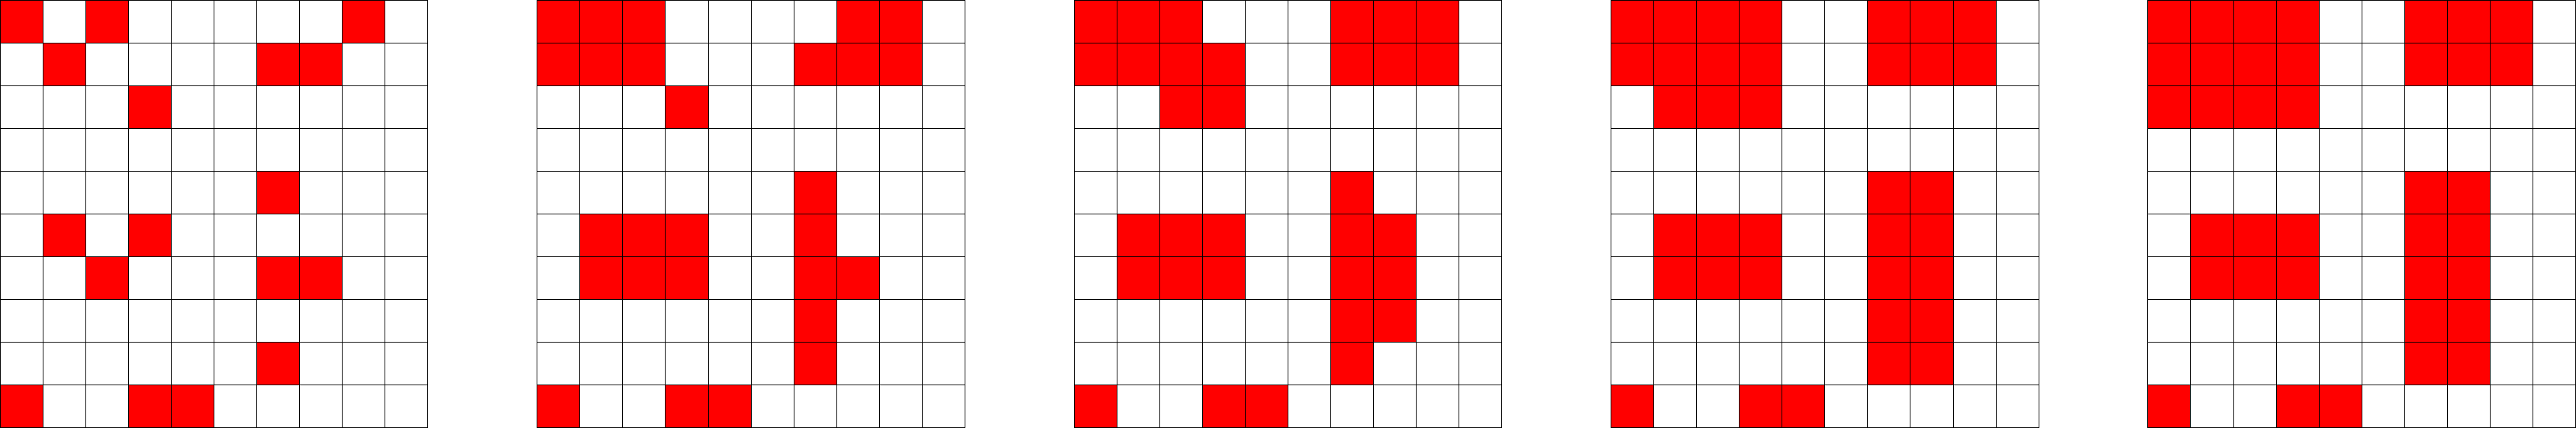
\includegraphics[width=\textwidth]{figures/1/simple_puzzle.pdf}
\caption{An arbitrary set of initially infected cells in the $10 \times 10$ lattice, and the stages of infection.}
\label{fig:simple_puzzle}
\end{figure} 

Before we present the solution,
%(which is particularly elegant and satisfying, and the reader is encouraged to play around with this problem on their own and get a feel for the behavior), 
let us take a moment to examine some properties of infectious sets and attempt to characterize what attributes might correspond to lethality. It should not take too long to observe that if an initial infection is in some way ``spread too thinly," then it will be unable to jump between infected areas, leading to gaps in infection, which we refer to as \emph{immune regions}. The perimeter of the lattice is particularly susceptible to this, as vertices there have fewer neighbors from whom they might be exposed. Heuristically, then, a lethal set must have the ability to effectively span the entire lattice, and must be particularly virulent along the perimeter. 

With this criteria in mind, we are able to make some educated guesses regarding the specific structure of sets that are likely to be lethal. In particular, we would like to consider the two starting infections illustrated in Figure \ref{fig:two_infections}. Notice that while Figure \ref{fig:two_infections} (\subref{fig:two_infections_b}) has far fewer perimeter infections, both (\subref{fig:two_infections_a}) and (\subref{fig:two_infections_b}) manage to form continuous bands of infected cells that appear to span the entire lattice after one step. Indeed, this fits with our notion of immune regions (or lack thereof), and we see that both infections will continue to propagate outwards from these bands until all cells become infected.

\begin{figure}[]
\centering
\begin{subfigure}{0.45\textwidth}
	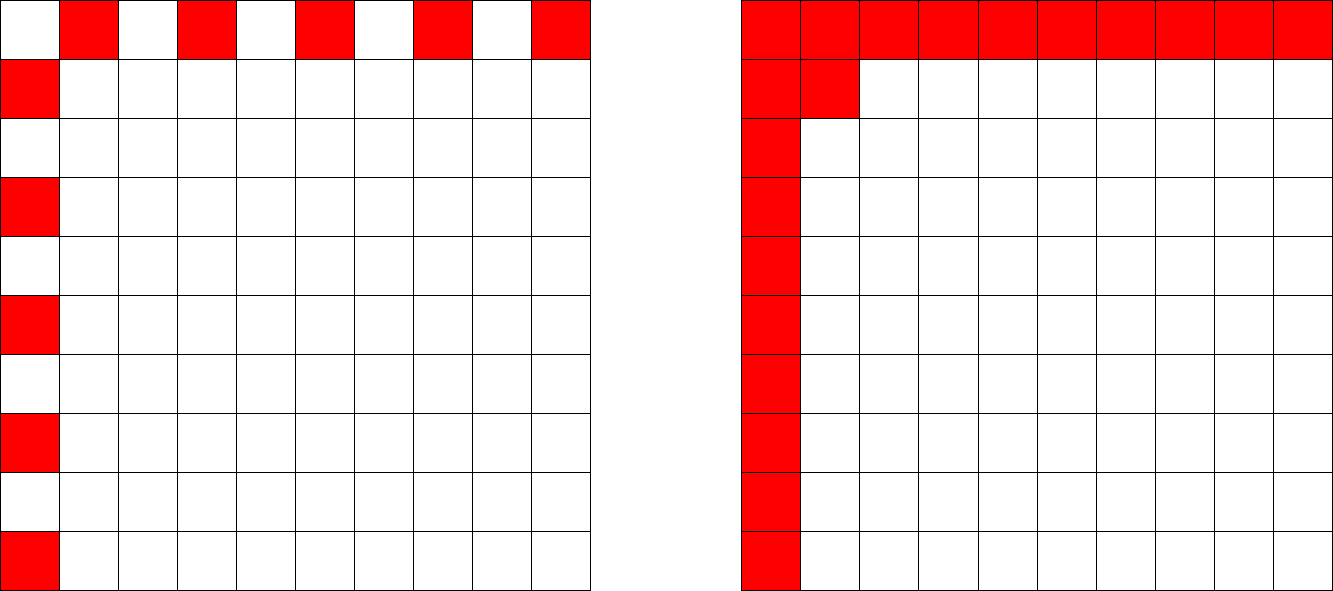
\includegraphics[width=\textwidth]{figures/1/two_infections_a.pdf}
	\caption{Perimeter construction.}
	\label{fig:two_infections_a}
\end{subfigure} \hfill%
\begin{subfigure}{0.45\textwidth}
	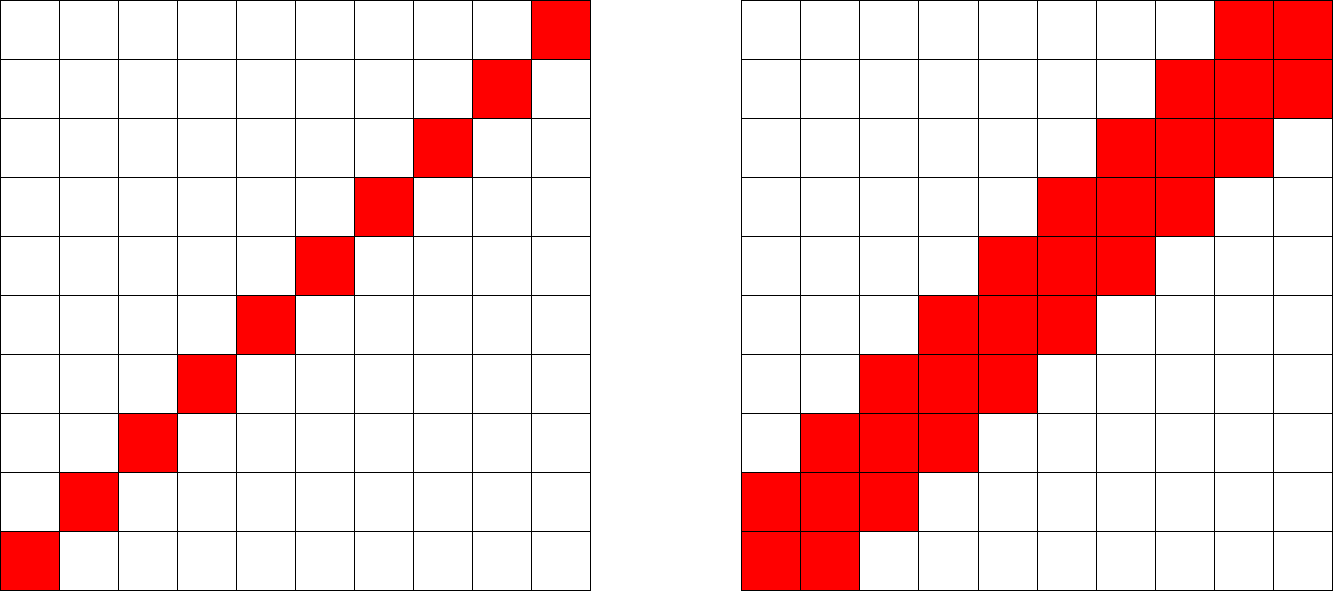
\includegraphics[width=\textwidth]{figures/1/two_infections_b.pdf}
	\caption{Diagonal construction.}
	\label{fig:two_infections_b}
\end{subfigure}
\caption{Two lethal sets and their resulting infections after one time-step.}
\label{fig:two_infections}
\end{figure} 

It is clear from Figure \ref{fig:two_infections} that we may obtain lethal sets on the $n \times n$ lattice of size $n$ by simply infecting the diagonal. What is less obvious is whether it is possible to improve upon this result. Perhaps the most natural first attempt at this is to remove an infection from one of the cells along the diagonal. However, this seems to form an immune region containing the removed cell. After some experimentation, one begins to believe it impossible to simultaneously satisfy the heuristic that a starting infection must span the lattice, while also using fewer than $n$ initial infections. The question therefore becomes: how do we prove it?

Consider the cumulative perimeter of infected regions. For a given infectious set $A$, let $P(A)$ be the total perimeter of the infected regions of $A$. Let $A_0$ be an initial infection, and observe that $P(A_0) \leq 4 |A_0|$. (This bound is only tight if no two infected cells are adjacent. Otherwise, the edge between such cells lies within the infected region, and cannot contribute to the infection's perimeter.) Observe that for any uninfected cell to become infected, it must abut at least two infected cells. Upon infection, the edges adjacent to these cells no longer lie on the infection's perimeter; additionally, the remaining edges of this newly infected cell contribute at most $2$ to this perimeter. All told, after infection, $P(A_1) \leq P(A_0)$. 

If we suppose that $A_0$ is a lethal set, then at some point in time, the entire grid will become infected. This infection will have a perimeter $4n$. Since this perimeter did not increase, $A_0$ must have originally had a perimeter of at least $4n$. Since each cell in $A_0$ can contribute at most $4$ to this perimeter, it must be the case that $|A_0| \geq n$. Our diagonal construction shows that $|A_0| \leq n$, and so we are able to conclude that $n$ is best possible.

This proof is an instance of the famous \emph{perimeter argument}, which has belonged to bootstrap percolation folklore since at least the work of Pete \cite{pete:1997}. In the following section, we present generalizations of this argument to higher dimensional rectangular grids.

\section{Bootstrap Percolation}

%Before presenting a proof, let us take a moment to formally define the process described above and develop some useful notation. 
The study of such cellular infection spread in grids (and, more generally, in graphs) is known in the literature as \emph{bootstrap percolation}, and was introduced in the 1970s by Chalupa et al. \cite{chalupa:1979} as a simplified model for the behavior of ferromagnetic fields. In their original 1979 paper, the authors research the stable structure of probabilistically selected initial infections. While this differs from the problem posed in Question \ref{que:simple_puzzle}, the rules for the spread of infection and its broad behavior remain the same. It is worth noting that a large portion of contemporary research on bootstrap problems is focused on questions of probabilistic nature; while these problems are certainly interesting and of merit, they do not fall within the scope of this thesis. Rather, we shall focus on those problems where we have specific control over the structure of the initial infections; in particular, we aim to determine the smallest lethal set on the Cartesian product of paths and cycles. 

Let us now define the problem in concrete terms. Let $G$ be a graph, let $r \geq 0$ and let $A_0 \subseteq V(G)$ be a set of initially infected vertices. Iteratively, infect those vertices of $G$ with at least $r$ infected neighbors. For all $t > 0$, let $A_t$ be the set of infected vertices at time step $t$. We then have
$$A_t = A_{t-1} \cup \{v \in V(G) : |N_G(v) \cap A_{t-1}| \geq r\},$$
where $N_G(v)$ is the set of vertices adjacent to $v$ in $G$. We define the \emph{closure} of $A_0$ under $r$-neighbor bootstrap percolation to be $[A_0] = \bigcup_{t=0}^{\infty} A_t$. We say that $A_0$ \emph{percolates} or is \emph{lethal} if $[A_0] = V(G)$. We define the smallest lethal set in a graph $G$ under $r$-neighbor bootstrap percolation by the quantity $m(G,r)$. We note that under these rules, it is not possible for vertices to become uninfected.

While it is possible to study bootstrap percolation on any graph $G$, much of the contemporary research focuses on multidimensional grids \cite{something}. We therefore introduce the following notation. For all $n \in \mathbb{N}$, let $[n] = \{1, 2, \dots, n\}$. Let the grid graph with vertex set $\prod_i^d [a_i]$ be denoted by $\prod_i^d [a_i]$. Note that $\prod_i^d [a_i] = P_{a_1} \square \cdots \square P_{a_d}$. Furthermore, define:
$$m(a_1, \dots, a_d, r) = m(\prod_i^d [a_i], r).$$

There are a number of natural generalizations of the problem posed in Question \ref{que:simple_puzzle}. In this thesis, we discuss those obtained by varying the structure of $G$ and the value of $r$. Below, we outline some of the existing results for graphs that are the Cartesian product of paths and cycles, and $r \in \{0, 1, 2, 3\}$. These results are summarized in Table \ref{tab:known_bounds}.

\begin{table}[]
\centering
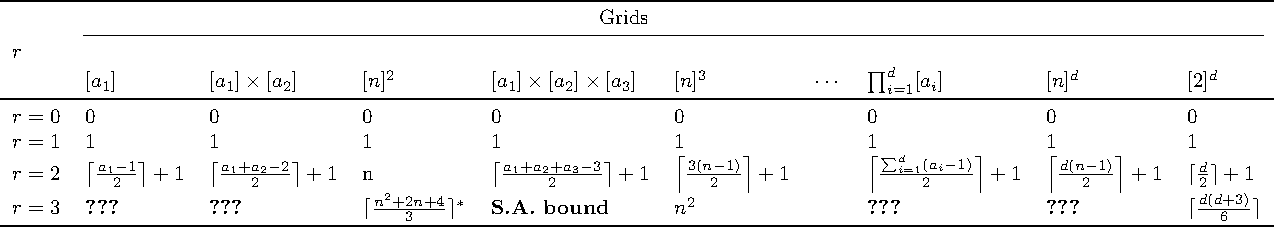
\includegraphics[width=\textwidth,origin=c]{tables/1/known_bounds.pdf}
\caption{A summary of known bootstrap percolation results for grids and the torus, $r \in \{0,1,2,3,d\}$.}
\label{tab:known_bounds}
\end{table} 

\subsection{Results on grids and tori}
\label{sec:result_summary}

In this section, we highlight major bootstrap percolation results on grids and tori. Some of the following bounds are not tight and require supplemental constructions, which are often difficult to obtain. We further sub-divide this discussion into results on the grid (of which there are many), and results on the torus (of which there are few).

\subsubsection{Grids}

From the puzzle posed in Question \ref{que:simple_puzzle}, we readily obtain variant problems by altering three parameters: the size and shape of the grid $G$, the grid's dimension $d$, and the threshold number of neighbors $r$. We examine each of these problems in turn.

In the prior discussion of the perimeter argument, we showed that for square grids $[n]^2$, $m([n]^2, 2) \geq n$, and verified this to be tight with a diagonal construction. The following result (attributed to Pete) generalizes this result to all rectangular grids $[a_1] \times [a_2]$. A proof is included for completeness. 

\begin{thm}
\label{thm:perimeter_rects}
For $a_1, a_2 \geq 1$,
$$m(a_1,a_2,2) = \ceil*{\frac{a_1+a_2-2}{2}}+1.$$
\end{thm}

\begin{proof}
We obtain a lower bound on $m(a_1,a_2,2)$ by applying the perimeter argument. Note that the perimeter of the $a_1 \times a_2$ grid is $2(a_1+a_2)$, and so the $m(a_1,a_2,2) \geq \ceil*{\frac{a_1+a_2}{2}}$. (We take the ceiling because the size of infected sets must be integral. See Figure \ref{fig:sa_construction_2d}.) For the upper bound, we proceed by induction on $a_1+a_2$. For $a_1+a_2 \leq 4$, the lethal sets in Figure \ref{fig:base_cases} match the lower bounds given by the perimeter argument (1, 2, 2, and 2, respectively). For $a_1+a_2 > 4$, suppose without loss of generality that $a_1 \leq a_2$, and so $a_2 \geq 3$. By hypothesis, $[a_1] \times [a_2-2]$ admits a lethal set $A_0$ at the perimeter bound. We show that $A_0$, plus the addition of any infection in the final column of $[a_1] \times [a_2]$, is lethal and matches the perimeter bound. 

Observe that $A_0$ infects all vertices of $[a_1] \times [a_2]$, apart from the final two columns. The additional vertex in the final column is then sufficient to infect all remaining healthy vertices. Finally, by incrementing $a_2$ by two, the perimeter bound is incremented by exactly one. This completes the proof.
\end{proof}

\begin{figure}[]
\centering
\begin{subfigure}{0.03\textwidth}
	
\includegraphics[width=\textwidth]{figures/1/1x1x1.pdf}
\end{subfigure} \hfill%
\begin{subfigure}{0.064\textwidth}
	
\includegraphics[width=\textwidth]{figures/1/1x2x1.pdf}
\end{subfigure} \hfill%
\begin{subfigure}{0.1\textwidth}
	
\includegraphics[width=\textwidth]{figures/1/1x3x1.pdf}
\end{subfigure} \hfill%
\begin{subfigure}{0.06\textwidth}
	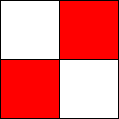
\includegraphics[width=\textwidth]{figures/1/2x2x1.pdf}
\end{subfigure}
\caption{Tight constructions for lethal sets where $a_1+a_2 \leq 4$.}
\label{fig:base_cases}
\end{figure} 

Let us take a moment to examine the issue of integrality in the perimeter bound. Non-integrality occurs either when adjacent vertices are infected in the same generation, or when a vertex is infected by more than $r$ neighbors. Note that in both cases, this decreases the perimeter of infection. One way to think about this is to consider each vertex as having ``infectious potential": vertices $v \in A_0$ can infect up to $d(v)$ healthy vertices, whereas vertices $v \in A_i$ for $i > 0$ can infect at most $d(v) - r$. An integral perimeter bound mandates that each vertex realize its potential, whereas a non-integral bound leaves a small margin for error. Figure \ref{fig:sa_construction_2d_a} illustrates the integral case, where each cell is infected by exactly two neighboring cells; this condition ensures that $P(A_i) = P([A_0])$ for all $i$. Conversely, in Figure \ref{fig:sa_construction_2d_b}, the cell demarcated with an ``X" experiences infection on three sides, thereby reducing its infectious potential. The existence of such a cell is guaranteed by the fact the perimeter bound in this case is non-integral. 

\begin{figure}[]
\centering
\begin{subfigure}{0.4\textwidth}
	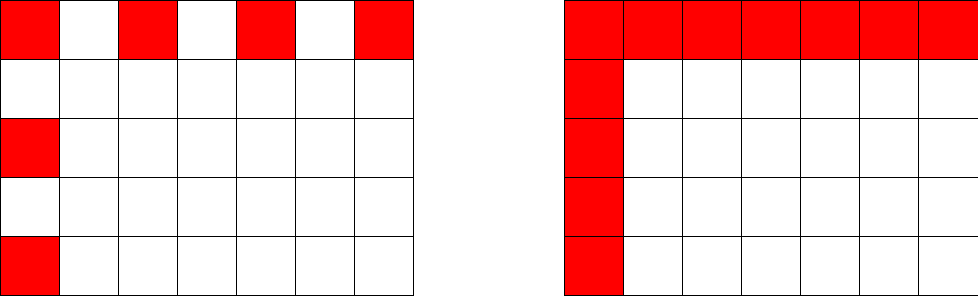
\includegraphics[width=\textwidth]{figures/1/5x7x1.pdf}
	\caption{$a+b \equiv 0 \pmod 2$}
	\label{fig:sa_construction_2d_a}
\end{subfigure} \hfill%
\begin{subfigure}{0.45\textwidth}
	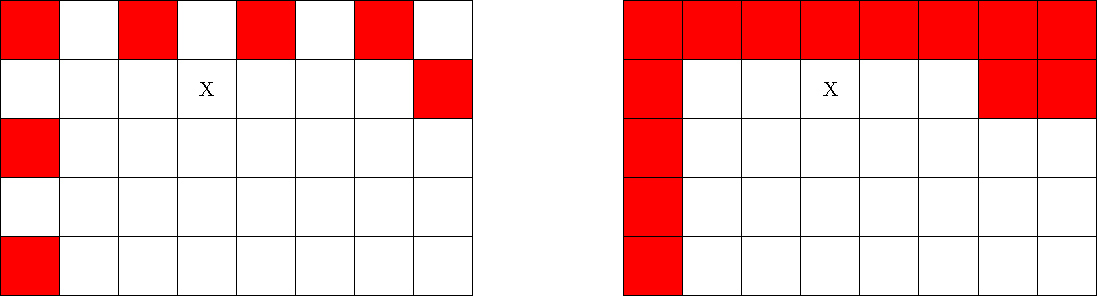
\includegraphics[width=\textwidth]{figures/1/5x8x1.pdf}
	\caption{$a+b \equiv 1 \pmod 2$}
	\label{fig:sa_construction_2d_b}
\end{subfigure}
\caption{Tight constructions for lethal sets on the $[a] \times [b]$ grid.}
\label{fig:sa_construction_2d}
\end{figure} 

We can further generalize for the case of $r=2$. In 2006, Balogh and Bollobas \cite{balogh:2006} proved the following general form of Theorem \ref{thm:perimeter_rects} for all $d$-dimensional hypercubes $(a_1, \dots, a_d)$, $a_i \geq 1$:

\begin{thm}[Balogh]
\label{thm:complete_r_2}
For $d \geq 1$ and $a_1, \dots, a_d \geq 1$, 
$$m(a_1, \dots, a_d, 2) = \ceil*{\frac{\sum_{i=1}^d (a_i-1)}{2}}+1.$$
\end{thm}

Theorem \ref{thm:complete_r_2} completes the picture for infections with a threshold of two on grids. The next question is whether similar results exist for larger $r$. Unfortunately, while generalizing to $d$-dimensional grids yields nice results for $r=2$, attempts to obtain a holistic understanding of $m(a_1, \dots, a_d, r)$ for arbitrary $r$ have been largely fruitless. Even the case of $r=3$ remains stubbornly inaccessible for nearly all large $d$. However, certain breakthroughs have been made in the following circumstances: $d=2$, $d=3$, and $G=[2]^d$.

We first consider 3-neighbor percolation on two-dimensional square grids. In 2021, Benevides et al. proved that 
$$m(n,n,3) = \ceil*{\frac{n^2+2n+4}{3}}$$
for even $n$, and 
$$\ceil*{\frac{n^2+2n}{3}} \leq m(n,n,3) \leq \ceil*{\frac{n^2+2n}{3}} + 1$$
for odd $n$. Additionally, they showed that these bounds are tight for odd $n$: if $n = 5 \pmod 6$, or $n = 2^k - 1$ for some $k \in \mathbb{N}$, then $m(n,n,3) = \ceil{\frac{n^2+2n}{3}}$; and if $n \in \{9,13\}$, then $m(n,n,3) = \ceil{\frac{n^2+2n}{3}} + 1$. Constructions that achieve this bound are illustrated in Chapter 7. We add to this picture with the following theorem, proven in Chapter 6, and corollary:

\begin{thm}
\label{thm:2d_rectangle}
Suppose that $a, b \geq 1$ such that
$$m(a,b,3) = \frac{2ab+a+b}{3}.$$
Then there exists $k \geq 1$ such that $a=b=2^k-1$.
\end{thm}

\begin{cor}
For all $n \geq 1$,
$$ m(n,n,3) =
\begin{cases} 
      \ceil*{\frac{n^2+2n+4}{3}} & n \equiv 0 \pmod 2 \\
      \frac{n^2+2n}{3} & n = 2^k-1, \; k \in \mathbb{N} \\
      \frac{n^2+2n+1}{3} & n \equiv 5 \pmod 6 \\
      \frac{n^2+2n+3}{3} & \text{otherwise.}
   \end{cases}
$$
\end{cor}

\begin{proof}
The first three cases follow from Theorem 1 of \cite{benevides:2021} and the observation that if $n \equiv 5 \pmod 6$, then $\ceil{\frac{n^2+2n}{3}} = \frac{n^2+2n+1}{3}$. In the final case, $n$ is congruent to either 1 or 3 modulo 6. This implies that $n^2 + 2n$ is divisible by three. From Theorem 1 of \cite{benevides:2021}, we have that $m(n,n,3) \leq \frac{n^2+2n+3}{3}$. Furthermore, since $n$ is not of the form $2^k-1$, it follows from Theorem \ref{thm:2d_rectangle} that $m(n,n,3) > \frac{n^2+2n}{3}$. Therefore, $m(n,n,3) = \frac{n^2+2n+3}{3}$.
\end{proof}

This result resolves the question of the minimum lethal set for two dimensional square grids. For the more general case of rectangular grids, the problem remains unsolved. However, we are able to achieve an upper bound of $m(a,b,3) \leq \ceil{\frac{ab+a+b+6}{3}}$ and a lower bound (described below) of $m(a,b,3) \geq \ceil{\frac{ab+a+b}{3}}$, for all $a,b > 1$. Further discussion of these results can be found in Chapter 6.

One significant and well-known result for 3-neighbor percolation on two- and three-dimensional grids is the following lower bound, taken as a three-dimensional analogue of the perimeter bound. This result is referenced frequently throughout this document, and referred to interchangeably as the \emph{surface area} or \emph{SA bound}. We prove the statement in full generality, while noting that we only make use of the case where $d=3$. We also note that, like the perimeter bound, the following proof belongs to bootstrap percolation folklore, and appears to have been first published in 1997 by Balogh and Pete \cite{balogh_and_pete}.

\begin{thm}
\label{thm:sa_bound}
For any $d \geq 1$ and $a_1, a_2, \dots, a_d \geq 1$, 
$$m(a_1,a_2, \dots, a_d,d) \geq \frac{\sum_{j=1}^d \prod_{i \neq j} a_i}{d}.$$
\end{thm}

\begin{proof}
We apply the same invariant strategy presented in the perimeter argument. For simplicity, consider $\prod_{i=1}^d[a_i]$ to be embedded within the larger graph $\prod_{i=1}^d \{0, \dots, a_i + 1\}$. Note that in $\prod_{i=1}^d \{0, \dots, a_i + 1\}$, each vertex $v \in \prod_{i=1}^d[a_i]$ has degree $2d$. Let $A_0$ be a lethal set in $\prod_{i=1}^d[a_i]$ under the $d$-neighbor bootstrap process. Let $A_t$ be the set of infected vertices in $\prod_{i=1}^d[a_i]$ at generation $t$. Denote by $m_t$ the number of edges between vertices $u \in A_t$ and $v \in \prod_{i=1}^d[a_i] \setminus A_t$. %We show that the sequence $m_0, m_1, m_2, \dots$ is monotonically decreasing. 
We show that $m_{t-1} \geq m_t$ for all $t> 0$. 

%Let $N = |A_t - A_{t-1}|$, and let $v_1, \dots, v_N$ be an arbitrary ordering on the vertices of $A_t \setminus A_{t-1}$. 
By definition, each vertex $v \in A_t \setminus A_{t-1}$ has at least $d$ neighbors in $A_{t-1}$. Therefore, since $d(v) = 2d$, $v$ has no more than $d$ neighbors outside of $A_t$. This implies that the number of edges from $A_{t-1} \cup \{v\}$ to $\prod_{i=1}^d[a_i] \setminus A_{t-1} \cup \{v\}$ cannot exceed $m_{t-1}$. Furthermore, this holds for every vertex $v \in A_{t-1}$, and so $m_{t-1} \geq m_t$. 

Since $A_0$ is lethal, we have that 
$$2d|A_0| \geq m_0 \geq m_1 \geq \dots \geq 2 \sum_{j=1}^d \prod_{i \neq j} a_i,$$ 
where the final expression gives the total number of edges between the fully infected grid and the surrounding larger grid. Dividing through by $2d$ gives the result.
\end{proof}

We note that the prior argument is precisely the same as the so-called perimeter argument outlined on Page 2. Here, the quantity $m_t$ is a $d$-dimensional analogue of the perimeter of infection $P(A_t)$ at time-step $t$, and the lower bound
$$2\sum_{j=1}^d \prod_{i \neq j} a_i$$
is the $d$-dimensional ``perimeter" of the grid. Again, observe that equality can only be obtained when no vertices of $A_0$ are adjacent, and all vertices $v \in A_{t>0}$ are infected by exactly $d$ neighbors. Any imprecision causes a reduction in ``perimeter" of two units, corresponding to a $1/d$ increase in the bound. 

The primary aim of this thesis is to prove that the surface area bound is tight for sufficiently large grids when $r=3$. This process employs a number of general constructions (discussed in Chapter 7), as well as a recursive strategy (Chapter 3). In Chapter 5, we prove the following result:

\begin{thm}
\label{thm:main_result}
For all $a_1, a_2, a_3 \geq 11$, 
$$m(a_1,a_2,a_3,3) = \ceil*{\frac{a_1a_2+a_2a_3+a_1a_3}{3}}.$$
\end{thm}

Unfortunately, the complete resolution of the $r=3$ case on grids remains elusive. Tight constructions exist for cubes $[n]^3$ and hypercubes $[2]^d$, but in general bounds are difficult to obtain. Worse, for $r>3$, the only additional result beyond the surface area bound addresses the very specific case of $r$-dimensional cubes. Open problems abound.

\subsubsection{Tori}

In addition to varying the parameters $r$ and $d$, we might also change the very structure of $G$. It is natural to shift from grids (the Cartesian product of paths) to tori (the Cartesian product of cycles). In fact, it could be argued that bootstrap percolation on the torus is \emph{more} natural than the grid, since tori are regular and grids are not. This problem has been studied by Benevides et al. In 2021, they obtained the following lower bound for the Cartesian product of two cycles \cite{benevides:2021}. Their proof is included here for completeness.

\begin{thm}
\label{thm:torus_lb}
For $a, b \geq 1$,
$$m(C_a \square C_b,3) \geq \ceil*{\frac{ab +1}{3}}.$$
\end{thm}

\begin{proof}
Let $G = C_a \square C_b$, and let $I$ be a lethal set on $G$. Let $H = V(G) \setminus I$, and note that $|H| = ab - |I|$. Let $m_{H}$ be the number of edges in the subgraph of $G$ induced by $H$, and $m_{IH}$ be the number of edges between vertices in $I$ and vertices in $H$. Note that $m_{IH}$ is similar to the notion of perimeter on a grid.

Observe that $G[H]$ must be cycle-free: cycles in $G[H]$ constitute immune regions, and contradict the lethality of $I$. Therefore, $G[H]$ is a forest, and so $m_H = |H| - c$, where $c$ is the number of components in $G[H]$. Additionally, note that $m_{IH} \leq 4|I|$, since $G$ is $4$-regular. Finally, observe that the total degree of $G[H]$ is $2m_H = 4|H| - m_{IH}$.

Chaining together these inequalities, we obtain:
\begin{align*}
4|I| \geq m_{IH} &= 4|H| - 2m_H \\
&= 4|H| - 2(|H| -c) = 2|H| + 2c \\
&= 2(ab-|I|) + 2c
\end{align*}
Combining like terms and simplifying, we have
$$|I| \geq \frac{ab +c}{3} \geq \frac{ab +1}{3}.$$
\end{proof}

Observe that the conditions $c \geq 1$ and $m_{IH} \leq 4|I|$ prevent us from obtaining strict equality. Specifically, if $I$ is lethal, $G[H]$ has one component, and no vertices in $I$ are adjacent, then $|I|$ is minimized. Note that these conditions are quite similar to those on grids; the specific difference is that equality in the bound on grids mandates that no vertex be infected by more than $r$ neighbors, whereas equality on three-dimensional tori requires this inefficiency be centered on one particular vertex. 

% other semi-related problems in bootstrap percolation
\section{Other Problems}

In this section, we provide a cursory overview of some other related areas of study in bootstrap percolation. We highlight problems regarding the number of iterations necessary to infect all vertices on a graph.

\section{Structure of this Thesis}

As stated by Theorem \ref{thm:main_result}, the primary goal of this thesis is to prove a tight bound for 3-neighbor bootstrap percolation on three-dimensional grids of sufficiently large size. This task requires the use of two major lemmas, as well as both original and previously published ideas and constructions. In an effort to present this material in a coherent manner, the paper is structured as follows. 

Chapters 2 and 3 are dedicated to building a conceptual and intuitive framework upon which to prove Theorem \ref{thm:main_result}. In Chapter 2, we categorize and present percolating sets on both divisible and non-divisible grids, and discuss the differences between these cases. In Chapter 3, we prove two lemmas allowing us to develop large families of lethal sets that match the surface area bound. 

Chapters 4 and 5 leverage the results of Chapter 3 to prove Theorem \ref{thm:main_result}. In Chapter 4, we show that all divisible grids $(a_1,a_2,a_3)$, $a_1 \leq a_2 \leq a_3$ admit lethal sets matching the SA bound, and in Chapter 5, we extend this result to all grids of size 11. Chapter 6 further builds on this, highlighting some new results for 3-neighbor percolation on grids of the form $(a_1,a_2,1)$.

Chapter 7 proves the constructions presented in Chapter 2.

Finally, Chapters 8, 9 and 10 wrap up the discussion with a summary of the programmatic techniques used to discover lethal sets, helpful software resources for future research, how the results of this thesis may be helpful in pursuit of results on the torus, and recommendations for future research in similar and related problems. 

% proof of perimeter bound and generalization to surface area bound
% "So we have a goal, and now the question becomes whether or not it is possible to obtain this goal in all cases through constructions."

% "We shall see that generally (and especially for large grids), it is possible to find constructions that percolate at the lower bound. However, some smaller cases seem to contain unavoidable regions of immunity."
% For this reason, it will be helpful to expand on our observations about immune regions and perimeter infections."
% discussion about the notion of immune regions

% Possible discussion of existing results, where our results fit into the literature and presentation of the table??

% Lay out the structure of this paper. 
% "We show that through a clever recursive construction we are able to obtain percolating sets at the lower bound for all grids of size at least 11, and at least 5 for divisibility cases."
% "We establish a set of cases for which the lower bound cannot be met, and present a best upper bound for these cases."
% 1. Introduction
% 2. Recursion
% 3. Divisibility cases
% 4. All cases
% 5. Thickness 1
% 6. Constructions
% 7. Visualization tool??
% 8. The torus?

% vvv ONE GIANT COMMENT vvv
% COMMENT
% COMMENT
% COMMENT
% COMMENT
% COMMENT
% COMMENT
% COMMENT
% COMMENT
\begin{comment}
In the following chapter, we lay out in formal terms those lemmas necessary to understand and prove Theorem \ref{thm:main_result}. In particular, we discuss the recursive technique that permits the construction of lethal sets on grids of arbitrary large size, as well as a number of characteristics of lethal sets. We distinguish between two types of grids--those with integral \emph{SA bound}, and those without--and show that it is possible obtain tight constructions on non-integral grids from integral grids. 

In Chapter 3, we prove that there exist lethal sets at the S.A. bound for all integral grids of size at least 5. This chapter makes significant use of a number of existing constructions, described in Chapter 6, as well as the recursive strategy introduced in Chapter 2. 

Chapter 4 extends the results of Chapter 3 to all grids of size at least 11 with non-integral surface area bound. 

Chapter 5 considers the specific case of grids of the form $(a,b,1)$, and answers a question posed in Benevides et al. \cite{benevides:2022} regarding the existence of tight lethal sets on non-square grids. 

Chapter 6 is dedicated to presenting and proving the lethality of sets on a number of grids, and families of grids. 

Chapter 7 discusses some of the programmatic techniques used to evaluate, examine and explore the behavior of percolating sets. 

Chapter 8 examines the problem of bootstrap percolation on the 3- and 4-torus, and presents a class of constructions within constant size of the lower bound. 

Chapter 9 presents open questions related to the results presented in this thesis, and provides some suggestions for future research.

% COMMENT

% r=0 and r=1
\subsection{$m(G,0)$ and $m(G,1)$} 

In the case where $r \in \{0,1\}$, the specific structure of $G$ is unimportant. We have the following results:

\begin{thm}
For all undirected, simple graphs $G$, $m(G,0) = 0$.
\end{thm}

\begin{proof}
As cells need not be adjacent to infections to become infected, $A_1 = V(G)$, and so $A_0 = \emptyset$ is lethal.
\end{proof}

\begin{thm}
Let $G$ be an undirected, simple graph with $c$ components. Then $m(G, 1) = c$.
\end{thm}

\begin{proof}
Let $A_0$ be lethal. As infections spread along all edges, it is both necessary and sufficient for each connected component of $G$ to contain exactly one vertex of $A_0$. Therefore, $|A_0| = m(G,1) = c$.
\end{proof}

% r=2
\subsection{$m(G,2)$} 

We consider three classes of generalizations: the Cartesian product of paths, the Cartesian product of cycles, and the Cartesian product of both. 

\subsubsection{Grid: $P_a \square P_b$}

Recall from the discussion of Question \ref{que:simple_puzzle} that $m(n, n,2) = n$, where the tight construction for the lower bound is given by a diagonal infection expanding laterally outwards. We generalize this result to all rectangular grids.

\begin{thm}
For $a, b \geq 1$,
$$m(a,b,2) = \ceil*{\frac{a+b-2}{2}}+1.$$
\end{thm}

\begin{proof}
We obtain a lower bound on $m(a,b,2)$ by applying the perimeter argument. Note that the perimeter of the $a \times b$ grid is $2(a+b)$, and so the $m(a,b,2) \geq \ceil*{\frac{a+b}{2}} = \ceil*{\frac{a+b-2}{2}}+1$. (We take the ceiling because the size of infected sets must be integral.) For the upper bound, we generalize the construction illustrated in Figure \ref{fig:two_infections_a} to rectangular grids. Consider two cases: $a+b \equiv 0 \pmod 2$ and $a+b \equiv 1 \pmod 2$ (see Figure \ref{fig:sa_construction_2d}). Note that in both cases, the initial infectious set $A_0$ is lethal. Furthermore, note that in Figure \ref{fig:sa_construction_2d_a}, $|A_0| = \frac{a+b}{2}$, and in Figure \ref{fig:sa_construction_2d_b}, $|A_0| = \ceil*{\frac{a+b}{2}}$. In both cases, this agrees with the perimeter bound.
\end{proof}

It is worth noting that the integrality condition on the perimeter bound corresponds exactly to the non-existence of cells that are infected by more than two neighbors. In Figure \ref{fig:sa_construction_2d_a}, each cell is infected by exactly two neighboring cells; this condition ensures that $P(A_i) = P([A_0])$ for all $i$. Conversely, in Figure \ref{fig:sa_construction_2d_b}, the cell demarcated with an ``X" experiences infection on three sides. The existence of such a cell is guaranteed by the fact the perimeter bound in this case is non-integral. 

\begin{figure}[]
\centering
\begin{subfigure}{0.4\textwidth}
	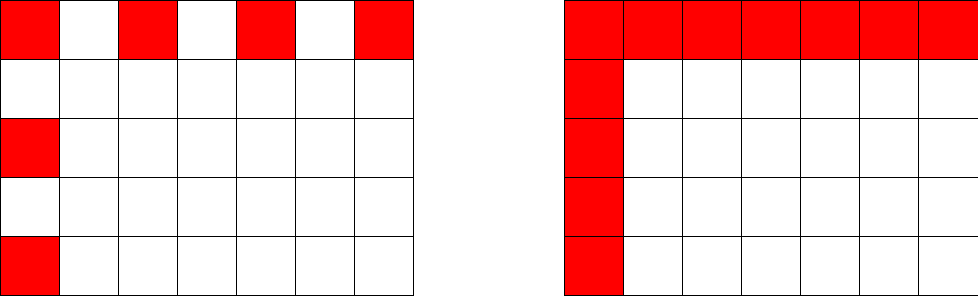
\includegraphics[width=\textwidth]{figures/1/5x7x1.pdf}
	\caption{$a+b \equiv 0 \pmod 2$}
	\label{fig:sa_construction_2d_a}
\end{subfigure} \hfill%
\begin{subfigure}{0.45\textwidth}
	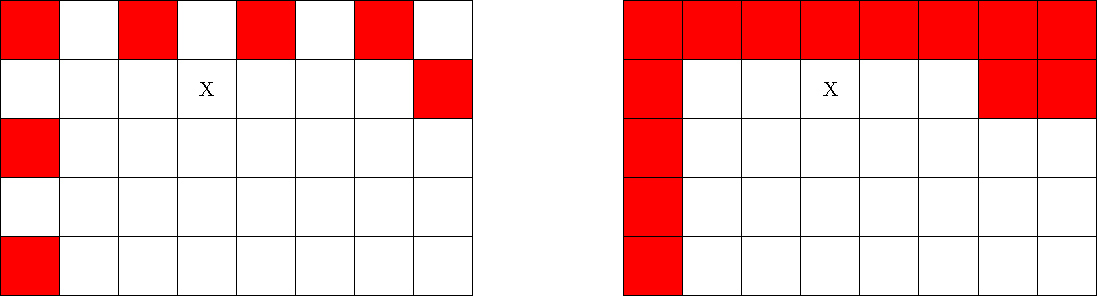
\includegraphics[width=\textwidth]{figures/1/5x8x1.pdf}
	\caption{$a+b \equiv 1 \pmod 2$}
	\label{fig:sa_construction_2d_b}
\end{subfigure}
\caption{Tight constructions for lethal sets on the $[a] \times [b]$ grid.}
\label{fig:sa_construction_2d}
\end{figure} 

\subsubsection{Grid: $P_a \square P_b \square \dots \square P_d$}

In a paper by Balogh and Bollobas \cite{balogh:2006}, the above result is generalized to all $d$-dimensional hypercubes $(a_1, \dots, a_d)$, $a_i \geq 1$. 

\begin{thm}
For $d \geq 1$ and $a_1, \dots, a_d \geq 1$, 
$$m(a_1, \dots, a_d, 2) = \ceil*{\frac{\sum_{i=1}^d (a_i-1)}{2}}+1.$$
\end{thm}

% r=3
\subsection{$m(G,3)$} 

We discuss a further generalization of the perimeter argument to higher dimensions. We show that this argument allows us to obtain nice bounds on 3-neighbor percolation in two and three-dimensional grids. We give a lower bound on the size of lethal sets in the 3-torus and 4-torus. We highlight the main theorem of this thesis.

\subsubsection{Grid: $P_n \square P_n$}

In 2021, Benevides et al. proved that 
$$m(n,n,3) = \ceil*{\frac{n^2+2n+4}{3}}$$
for even $n$, and 
$$\ceil*{\frac{n^2+2n}{3}} \leq m(n,n,3) \leq \ceil*{\frac{n^2+2n}{3}} + 1$$
for odd $n$. Additionally, they showed that these bounds are tight for odd $n$: if $n = 5 \pmod 6$, or $n = 2^k - 1$ for some $k \in \mathbb{N}$, then $m(n,n,3) = \ceil{\frac{n^2+2n}{3}}$; and if $n \in \{9,13\}$, then $m(n,n,3) = \ceil{\frac{n^2+2n}{3}} + 1$. Constructions that achieve this bound are illustrated in Chapter 5. We add to this picture with the following theorem, proven in Chapter X, and corollary:

\begin{thm}
\label{thm:2d_rectangle}
Suppose that $a, b \geq 1$ such that
$$m(a,b,3) = \frac{2ab+a+b}{3}.$$
Then there exists $k \geq 1$ such that $a=b=2^k-1$.
\end{thm}

\begin{cor}
For all $n \geq 1$,
$$ m(n,n,3) =
\begin{cases} 
      \ceil*{\frac{n^2+2n+4}{3}} & n \equiv 0 \pmod 2 \\
      \frac{n^2+2n}{3} & n = 2^k-1, \; k \in \mathbb{N} \\
      \frac{n^2+2n+1}{3} & n \equiv 5 \pmod 6 \\
      \frac{n^2+2n+3}{3} & \text{otherwise.}
   \end{cases}
$$
\end{cor}

\begin{proof}
The first three cases follow from Theorem 1 of \cite{benevides:2021} and the observation that if $n \equiv 5 \pmod 6$, then $\ceil{\frac{n^2+2n}{3}} = \frac{n^2+2n+1}{3}$. In the final case, $n$ is congruent to either 1 or 3 modulo 6. This implies that $n^2 + 2n$ is divisible by three. From Theorem 1 of \cite{benevides:2021}, we have that $m(n,n,3) \leq \frac{n^2+2n+3}{3}$. Furthermore, since $n$ is not of the form $2^k-1$, it follows from Theorem \ref{thm:2d_rectangle} that $m(n,n,3) > \frac{n^2+2n}{3}$. Therefore, $m(n,n,3) = \frac{n^2+2n+3}{3}$.
\end{proof}

This result resolves the question of the minimum lethal set for two dimensional square grids. For the more general case of rectangular grids, the problem remains unsolved. However, we are able to achieve an upper bound of $m(a,b,3) \leq \ceil{\frac{ab+a+b+6}{3}}$ for all $a,b > 1$. Further discussion of these results can be found in Chapter X.

\subsubsection{Grid: $P_a \square P_b \square P_c$}

%Observe that the surface area bound presented above applies directly to 3-dimensional grids. State the main theorem of this thesis. 
Surprisingly, it is possible to extend the perimeter argument to higher dimensions \cite{przykucki:2019}. This provides a lower bound on $m(a_1,a_2,a_3,3)$ of $\ceil{\frac{a_1a_2+a_2a_3+a_1a_3}{3}}$. We refer to this quantity as the \emph{surface area bound}. In Chapters 2 and 3, we use a recursive strategy to prove that the surface area bound is met for all sufficiently large grids. 

\begin{thm}
\label{thm:main_result}
For all $a_1, a_2, a_3 \geq 11$, 
$$m(a_1,a_2,a_3,3) = \ceil*{\frac{a_1a_2+a_2a_3+a_1a_3}{3}}.$$
\end{thm}

\subsubsection{Grid: $P_a \square P_b \square \dots \square P_d$}

Do we have a bound here?

\subsubsection{Torus: $C_a \square C_b$}

A lower bound for the Cartesian product of two cycles is given in Benevides \cite{benevides:2021}. Their proof is included here for completeness.

\begin{thm}
\label{thm:torus_lb}
For $a, b \geq 1$,
$$m(C_a \square C_b,3) \geq \ceil*{\frac{ab +1}{3}}.$$
\end{thm}

\begin{proof}
Let $G = C_a \square C_b$, and let $I$ be a lethal set on $G$. Let $H = V(G) \setminus I$, and note that $|H| = ab - |I|$. Let $m_{H}$ be the number of edges in the subgraph of $G$ induced by $H$, and $m_{IH}$ be the number of edges between vertices in $I$ and vertices in $H$. Note that $m_{IH}$ is similar to the notion of perimeter on a grid.

Observe that $G[H]$ must be cycle-free: cycles in $G[H]$ constitute immune regions, and contradict the lethality of $I$. Therefore, $G[H]$ is a forest, and so $m_H = |H| - c$, where $c$ is the number of components in $G[H]$. Additionally, note that $m_{IH} \leq 4|I|$, since $G$ is $4$-regular. Finally, observe that the total degree of $G[H]$ is $2m_H = 4|H| - m_{IH}$.

Chaining together these inequalities, we obtain:
\begin{align*}
4|I| \geq m_{IH} &= 4|H| - 2m_H \\
&= 4|H| - 2(|H| -c) = 2|H| + 2c \\
&= 2(ab-|I|) + 2c
\end{align*}
Combining like terms and simplifying, we have
$$|I| \geq \frac{ab +c}{3} \geq \frac{ab +1}{3}.$$
\end{proof}

Observe that the conditions $c \geq 1$ and $m_{IH} \leq 4|I|$ prevent us from obtaining strict equality. Specifically, if $I$ is lethal, $G[H]$ has one component, and no vertices in $I$ are adjacent, then $|I|$ is minimized. 

\subsubsection{Torus: $C_a \square C_b \square C_c$}

Present the lower bound and note that we are able to obtain constructions within constant distance of this bound for arbitrarily large grids.

%In the context of question \ref{que:simple_puzzle}, $G = P_{10} \Osq P_{10}$, and our diagonal construction shows us that $m(2,G) \leq 10$. In general, we have observed that for $G = P_n \Osq P_n$, $m(2, G) \leq n$. Now, let us prove that the bound is, in fact, tight. 

\begin{prop}
\label{prop:tight_perimeter}
For all $n \geq 1$, 
$$m([n]^2, 2) = n.$$
\end{prop}

\begin{proof}
The upper bound follows from our diagonal construction in figure \ref{fig:two_infections} (\subref{fig:two_infections_b}). The lower bound is given by the famous ``perimeter argument". Consider the $n\times n$ grid $G$, given by $G = P_n \Osq P_n$. Let $A_0 \subseteq V(G)$ be a set of initially infected cells. We claim that the total perimeter of all infected regions in $G$ is monotonically decreasing as a function of the time-step $t$. Consider an arbitrary healthy cell $c$. In order for $c$ to become infected, at least two of its edges must abut infected cells. However, this implies that (upon infection of $c$) these edges are absorbed within the newly expanded infected region, thereby reducing the perimeter of infection by two. As $c$ contains at most two un-absorbed edges, the perimeter of infection cannot increase. 

Since a lethal set will infect the entire grid, and therefore have a final perimeter of infection of $4n$, it follows that the perimeter of infection of $A_0$ must be at least $4n$, and so $m([n]^2, 2) \geq n.$
\end{proof}

This proof appears in \cite{przykucki:2019}, although it has been an established result in bootstrap percolation ``folklore" for considerably longer. We should like to make a few additional observations. 

First, note that we have used the following three expressions to describe the same graph $G$:

\begin{center}
\begin{enumerate*}[label=\roman*),itemjoin={\qquad}]
\item $n \times n$
\item $P_n \Osq P_n$
\item $[n]^2.$
\end{enumerate*}
\end{center}
\vspace{0.2in}

\noindent The notation in (i) is useful when discussing the shape of low dimensional, asymmetric grids. We use the notation in (ii) to remind readers that the fundamental structure in bootstrap percolation problems is a graph, and to suggest possible extensions of the problem discussed in this thesis to other similar objects. The notation in (iii) is the standard way to describe the vertex set of a grid graph, and can readily be generalized to any dimension $d$ by writing $[n]^d$. In a slight abuse of notation, we use $[n]^d$ to represent the entire graph $G$, and draw edges between vertices that differ by exactly one in exactly one coordinate. 

Second, the fact that we have used the notation $[n]^2$ in Proposition \ref{prop:tight_perimeter} suggests that we can generalize to higher dimensional grids $[n]^d$. Indeed, simply observe that for a given hypercube cell to become infected, it must donate at least $d$ of its $2d$ hyperplane faces to the infected region, thereby at most maintaining the current $(d-1)$-perimeter of infection. The following theorem summarizes this result.  

\begin{thm}
\label{thm:square_sa_bound}
For all $n,d \geq 1$, 
$$m([n]^d, d) \geq n^{d-1}.$$
\end{thm}

More generally, denote by $(a_1, \dots, a_n)$ the grid graph with vertex set $V = \{(i_1,\dots,i_n) \mid i_1 \in [a_1], \dots, i_n \in [a_n]\}$, and edge set $E = \{uv \mid u,v \text{ differ by one in exactly one coordinate}\}$. The following theorem provides a general lower bound on the size of lethal sets for all such graphs. 

\begin{thm}
\label{thm:general_sa_bound}
Let $G = (a_1, \dots, a_d)$, for $a_1, \dots, a_d, d \geq 1$. Then:
$$m(G, d) \geq \text{ sum of products of all subsets of size d-1, divided by d}.$$
\end{thm}

\begin{proof}
The proof follows the same high-dimensional surface area argument outlined above. 
\end{proof}

We highlight the three-dimensional instance of Theorem \ref{thm:general_sa_bound} in Corollary \ref{cor:sa_bound}, as it will prove particularly useful in the following chapters. We refer to this bound as the \emph{surface area} or \emph{S.A. bound}.

\begin{cor}
\label{cor:sa_bound}
Let $G = (a, b, c)$, for $a, b, c \geq 1$. Then:
$$m(G, 3) \geq \ceil*{\frac{ab + bc + ca}{3}}.$$
\end{cor}

\begin{proof}
Follows directly from Theorem \ref{thm:general_sa_bound}.
\end{proof}

While it has been shown that tight constructions exist for grids of the form $[n]^d$, where $r=d$, the problem of determining the existence of similar constructions for rectangular grids remains unsolved. In this thesis, we focus our attention on the particular case of $d=3$ and show that $m(a,b,c, 3) = \ceil*{\frac{ab + bc + ca}{3}}$ for all $a,b,c \geq 11$. 

% Separation of two commented out sections
% COMMENT
% COMMENT
% COMMENT
% COMMENT
% COMMENT

The problem of bootstrap percolation was first introduced in the 1970s by Chalupa et al. \cite{chalupa:1979} as a simplified model for the behavior of ferromagnetic fields. In their original paper, the authors describe bootstrap percolation as the stabilization of a probabilistically occupied lattice, where each occupied site must be adjacent to at least $m$ occupied neighbors. A re-rendering of the examples given in the original 1979 paper is presented in figures 1 and 2. 

In this original problem, the authors are interested in the structural patterns of these stable arrangements. Put differently, given a set of randomly distributed occupants on a $d$-dimensional lattice, what configuration can we expect these occupied sites to fall into, subject to the constraint that each occupied site is adjacent to at least $m$ other occupants? In this construction, a probabilistically populated lattice is iteratively de-populated until it reaches a stable state. 

Alternatively, we might consider the behavior of a population as it grows, instead of shrinks. In this model, it is useful to consider the population as harboring an infection that steadily spreads from site to site, subject to population density. We shall consider these infections to take place on a graph, with vertices representing members of our population (sites), and edges indicating adjacency. In formal terms: let $G$ be a graph and $A_0 \subseteq V(G)$ be a set of initially infected vertices. Iteratively, at every time step, infect those vertices of $G$ with at least $r$ infected neighbors. For all $t > 0$, let $A_t$ be the set of infected vertices at time step $t$. We then have
$$A_t = A_{t-1} \cup \{v \in V(G) : |N_G(v) \cap A_{t-1} \geq r\},$$
where $N_G(v)$ is the set of vertices adjacent to $v$ in $G$. We define the \emph{closure} of $A_0$ under $r$-neighbor bootstrap percolation to be $[A_0] = \bigcup_{t=0}^{\infty} A_t$. This is analogous to the stable states introduced in \cite{chalupa:1979}. We say that $A_0$ \emph{percolates} or is \emph{lethal} if $[A_0] = V(G)$. We note that under these rules, it is not possible for vertices to become uninfected. 

Perhaps the most natural extremal question regarding $r$-neighbor bootstrap percolation is that of determining the size of the smallest percolating set $A_0 \subseteq V(G)$, for a given graph $G$. We represent this quantity by $m(G,r)$. There has been a great deal of work done on establishing the value of $m(G,r)$ for various classes of graphs and values of $r$ (see \{citations, citations, etc., etc.\}). These results are incompletely summarized in table \ref{tab:known_bounds}, and a selection of particularly noteworthy proofs are presented in detail in the following section.

\begin{table}[]
\centering
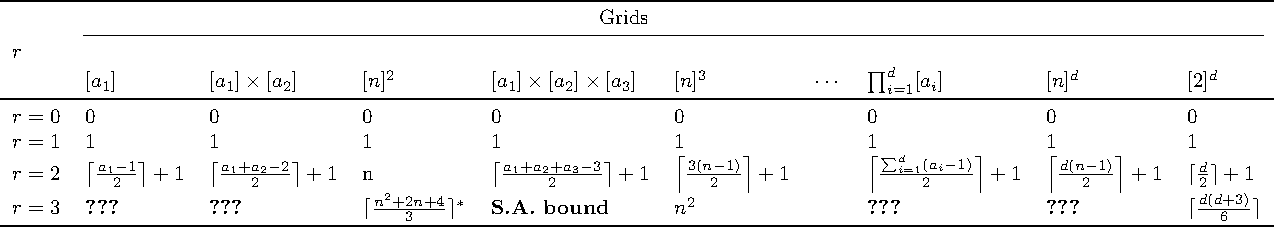
\includegraphics[width=\textwidth,origin=c]{tables/1/known_bounds.pdf}
\caption{A summary of known bootstrap percolation results for grids and the torus, $r \in \{0,1,2,3,d\}$.}
\label{tab:known_bounds}
\end{table} 

We end this introduction with the presentation of a delightful question about the cardinality of $2$-neighbor percolating sets on the two-dimensional lattice. The interested reader in encouraged to find a solution on their own; however, a proof of the result is presented at the beginning of the following section.
\begin{question}
Let $(n,n)$ represent the $n \times n$ lattice, given by $G = P_n \times P_n$. What is $m(n,n,2)$?
\end{question}

\section{Minimum percolating sets and bounds}

\subsection{Foundations}

Let us build some intuition for the behavior of percolating sets on the two-dimensional lattice. Figure \ref{fig:5x5x1} illustrates the percolation time-steps for an arbitrary initial infection on the graph $G=P_5 \times P_5$, where $r=2$. (In general, we shall refer to the $d$-dimensional lattice with sides $a_1, \dots, a_d$ as the $d$-tuple $(a_1, \dots, a_d)$. The standard notation is $\prod_{i=1}^d a_i$.) 

\begin{figure}[]
\centering
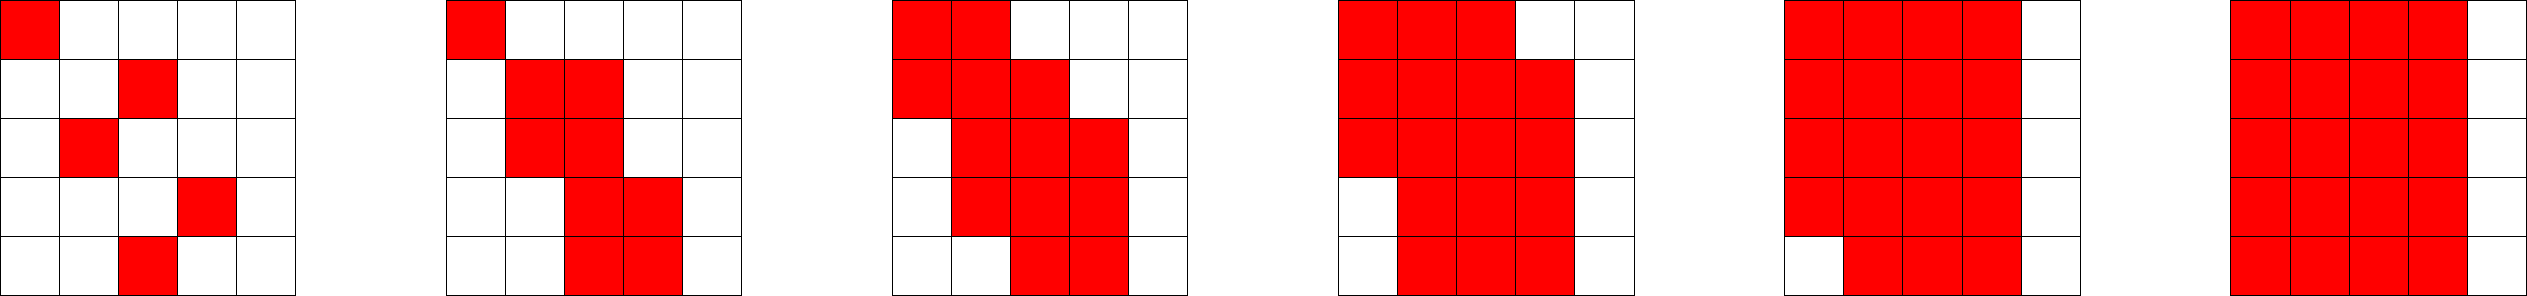
\includegraphics[width=\textwidth]{figures/1/5x5x1.pdf}
\caption{Percolation time-steps for an arbitrary initial infection on the $5 \times 5$ lattice, $r=2$.}
\label{fig:5x5x1}
\end{figure} 

Note that this configuration fails to infect the entire grid; that is, the initial infection is not lethal. Heuristically, this appears to be a consequence of the fact that infected cells are unable to access the healthy cells in the rightmost column. We might, therefore, hypothesize that an initial infection must somehow ``span" the entire lattice. A potential ``spanning" construction is illustrated in figure \ref{fig:5x5x1_improved}. Observe that at each time-step, the infection spreads out laterally from the initial diagonal. It is a simple exercise to verify that this construction is lethal on all $(n,n)$ grids for $r=2$. We also note that a similar construction is lethal on all $(n,m)$ grids for $r=2$ (figure \ref{fig:8x4x1}).

\begin{figure}[]
\centering
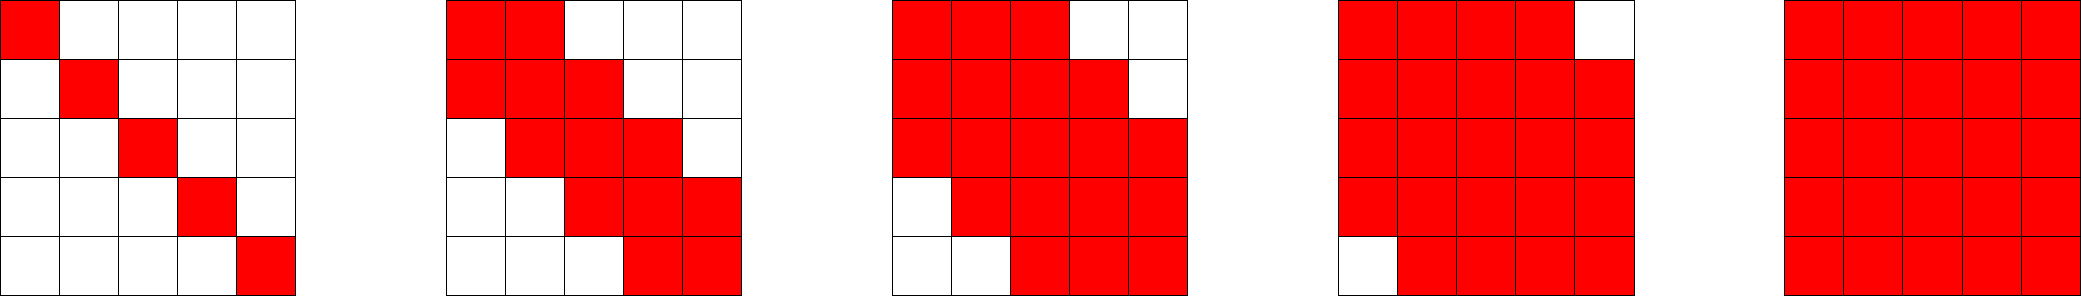
\includegraphics[width=\textwidth]{figures/1/5x5x1_improved.pdf}
\caption{Percolation time-steps for a ``spanning" initial infection on the $5 \times 5$ lattice, $r=2$.}
\label{fig:5x5x1_improved}
\end{figure} 

\begin{figure}[]
\centering
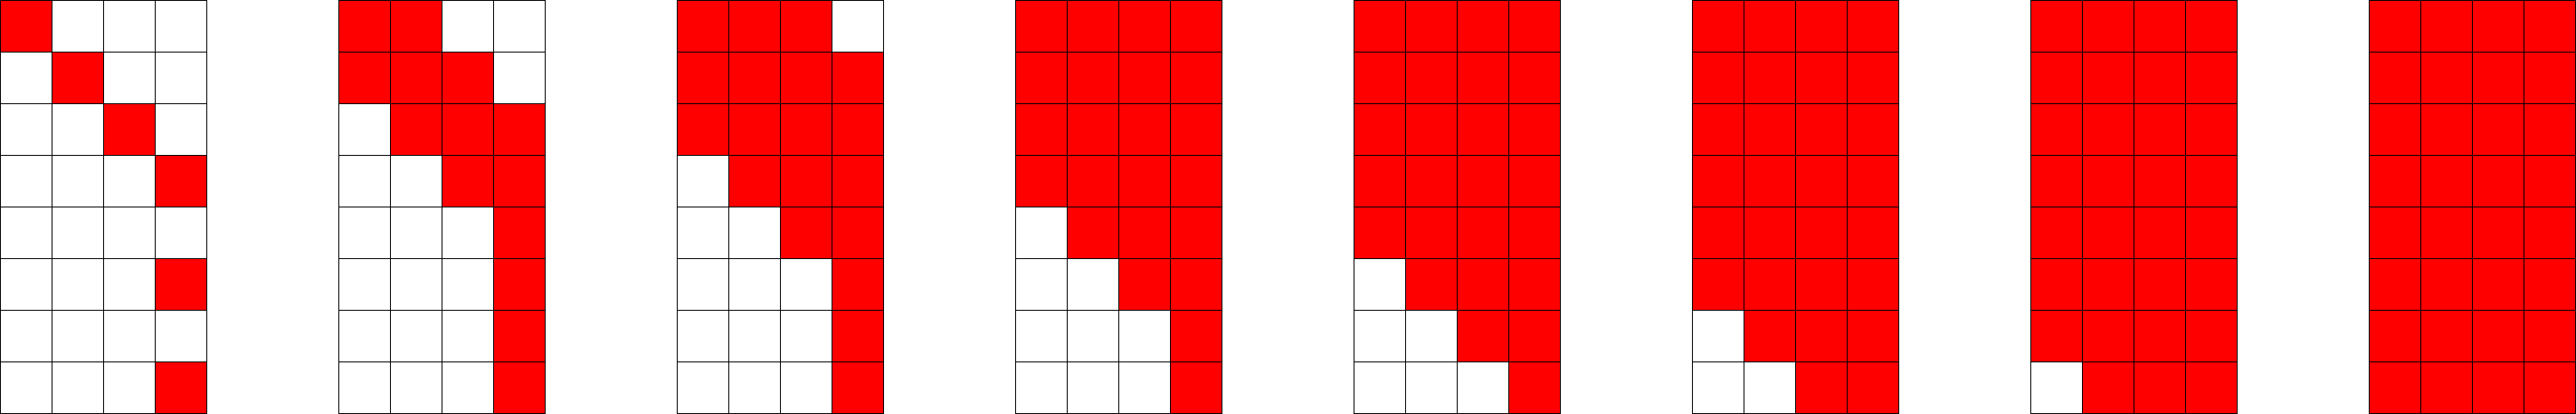
\includegraphics[width=\textwidth]{figures/1/8x4x1.pdf}
\caption{A lethal infection on the $8 \times 4$ lattice, $r=2$.}
\label{fig:8x4x1}
\end{figure} 

The $(n,n)$ construction can be generalized to any dimension. Specifically, we have:

\begin{prop}
\label{prop:nxn_lower_bound}
For all $n,d \geq 1$, 
$$m([n]^d, d) \leq n^{d-1}.$$
\end{prop}
This result has been known since at least Pete \cite{pete:1997}, although the particular constructions are difficult to render in general. The following proof (appearing in \cite{przykucki:2019}, but known in bootstrap percolation ``folklore" for much longer) elegantly shows that this bound is tight.

\begin{thm}
\label{thm:tight_perimeter}
For all $n,d \geq 1$, 
$$m([n]^d, d) = n^{d-1}.$$
\end{thm}

\begin{proof}
The upper bound follows from proposition \ref{prop:nxn_lower_bound}. The lower bound is given by a generalization of the famous ``perimeter argument". Suppose $d=2$ and consider an embedding of $G=[n]^d$ in the $n\times n$ grid. Let $A_0 \subseteq V(G)$ be a set of initially infected cells. We claim that the total perimeter of all infected regions in $G$ is monotonically decreasing as a function of the time-step $t$. Consider an arbitrary healthy cell $c$. In order for $c$ to become infected, at least two of its edges must abut infected cells. However, this implies that (upon infection of $c$) these edges are absorbed within the newly expanded infected region, thereby reducing the perimeter of infection by two. As $c$ contains at most two un-absorbed edges, the perimeter of infection cannot increase. 

Since a lethal set will infect the entire grid, and therefore have a final perimeter of infection of $4n$, it follows that the perimeter of infection of $A_0$ must be at least $4n$, and so $m([n]^2, 2) \geq n.$

The same argument generalizes nicely to higher dimensions. Simply observe that for a given hypercube cell to become infected, it must donate at least $d$ of its $2d$ hyperplane faces to the infected region, thereby at most maintaining the current $(d-1)$-perimeter of infection.
\end{proof}

We note that the perimeter argument extends directly to rectangular grids; however, the problem of obtaining tight constructions, should they exist, is largely unsolved and will be the main focus of this thesis. The following proposition, which we refer to informally as the \emph{surface area bound} or \emph{S.A. bound}, provides a lower bound on the size of lethal sets for $d$-dimensional rectangular grids where $r=d$.

\begin{prop}
\label{prop:SA_bound}
For $d \geq 1$ and $a_1, \dots, a_d \geq 1$,
$$m(a_1, \dots, a_d, d) \leq \frac{\sum_{i=1}^d \prod_{j \neq i} a_j}{d}.$$
\end{prop}

\begin{proof}
Observe that the expression
$$\frac{\sum_{i=1}^d \prod_{j \neq i} a_j}{d}$$
is precisely the high-dimensional perimeter of the grid graph $(a_1, \dots, a_d)$. The bound follows from the perimeter argument in theorem \ref{thm:tight_perimeter}. 
\end{proof}

In \{some chapter of this thesis\}, we will prove that this bound is tight in the case where $d=3$ and $d_1,d_2,d_3 \geq 8$. We fully expect that this bound can be incrementally diminished; however, we feel that such small improvements do not at this time justify the effort required to obtain additional constructions. 

In the remainder of this section, we shall present a number of additional bootstrap percolation results for different classes of grid graphs.

\subsection{Additional results}

Recall from the previous section that $m(n,n,2) = n$, where the tight construction for the lower bound is given by a diagonal infection expanding laterally outwards. In a paper by Balogh and Bollobas \cite{balogh:2006}, this result is generalized to all $d$-dimensional hypercubes $(a_1, \dots, a_d)$, $a_i \geq 1$. 

\begin{thm}
For $d \geq 1$ and $a_1, \dots, a_d \geq 1$, 
$$m(a_1, \dots, a_d, 2) = \ceil*{\frac{\sum_{i=1}^d (a_i-1)}{2}}+1.$$
\end{thm}

\begin{proof}
\end{proof}

As suggested by table \ref{tab:known_bounds}, general results become quite sparse for $r \notin \{2,d\}$. A nice result from Morrison and Noel resolves the question of $r=3$ for hypercubes $P_2^d$ of dimension $d \geq 3$. 

\begin{thm}
For $d \geq 3$ and $a_1 = \dots = a_d = 2$, 
$$m(a_1, \dots, a_d, 3) = \ceil*{\frac{d(d+3)}{6}}.$$
\end{thm}

\begin{proof}
\end{proof}

However, the issue of determining $m(a_1, \dots, a_d, r)$ is largely unresolved. Furthermore, good lower bounds for $r \neq d$ are conspicuously absent. 
\end{comment}
% ^^^ ONE GIANT COMMENT ^^^
% COMMENT
% COMMENT
% COMMENT
% COMMENT
% COMMENT



\chapter{Two Recursive Techniques}

In this chapter, we shall present two techniques for constructing large \emph{perfect} grids from smaller perfect grids. The first is a recursive technique that builds $d$-dimensional sets from $(d-1)$-dimensional components, while the second builds $d$-dimensional sets from smaller blocks of the same dimension. 

\section{The Three Walls Lemma}

\begin{lem}
\label{lem:walls}
Let $S$ be an infected set on $G = \prod_{i=1}^d [a_i]$. Let $\overline{S} = V(G) \setminus S$, and let $H = G[\overline{S}]$ be the subgraph of $G$ induced by $\overline{S}$. For $1 \leq k \leq a_j$, let $F_{j,k} = \prod_{i=1}^{j-1} [a_i] \times \{k\} \times \prod_{i=j+1}^{d} [a_i]$ be the $k$th face of $G$ in the $j$th dimension. If $H$ does not contain a path between $F_{j,1}$ and $F_{j,a_j}$, for all $1 \leq j \leq d$, then $G$ percolates.
\end{lem}

\begin{proof}
We proceed by induction on $|V(H)| = \prod_{i=1}^d a_i - |S|$. If $|V(H)| = 0$, then all vertices of $G$ are infected and we are done. Suppose $|V(H)| > 0$, and consider a connected component $Y$ of $H$. By hypothesis, for all $j \in [d]$, either $V(Y) \cap F_{j,1} = \emptyset$ or $V(Y) \cap F_{j,a_j} = \emptyset$ (or both). Suppose, without loss of generality, that $V(Y) \cap F_{j,a_j} = \emptyset$.
%Since $V(H) > 0$, there exists a $k_j < a_j$ such that $V(Y) \cap F_{j,k_j}$ is non-empty. 
For each $j \in [d]$, let $x_j$ be the maximum value such that $V(Y) \cap F_{j,x_j}$ is non-empty. Note that such an $x_j$ must exist since $|V(H)| > 0$. 

Consider the vertex $\vec{x} = (x_1, \dots, x_d) \in V(Y)$, and observe that 
$$\{\bigcup_{j \in [d]} F_{j,x_j+1}\} \cap  V(Y) = \emptyset.$$
In particular, note that $(x_1+1, x_2, \dots, x_d), \dots, (x_1, \dots, x_d+1) \in N_S(\vec{x})$. Therefore, $\vec{x}$ becomes infected. Furthermore, since $|V(H) \setminus \{\vec{x}\}| < |V(H)|$, the resulting graph percolates by induction. This completes the proof.
\end{proof}

\begin{cor}
\label{cor:walls}
Let $G$ be the grid graph $\prod_{i=1}^d [a_i]$. For each $j \in [d]$ and some $1 \leq k \leq a_j$, let 
$$M = \bigcup_{j,k} F_{j,k}$$
be a subset of the vertices of $G$ formed by the union of mutually orthogonal faces. If a set $S$ is lethal on $M$, then it is lethal on $G$. 
%Let $G$ be the grid graph $(a,b,c)$. If a set $A$ is lethal on three mutually orthogonal faces of $G$, then $A$ is lethal on $G$.
\end{cor}

\begin{proof}
Since $S$ is lethal on $M$, there exists a time $t$ where $M \subseteq A_t$. Therefore, for all $j \in [d]$, the graph $G[\overline{A_t}]$ cannot contain a path between $F_{j,1}$ and $F_{j,a_j}$. By Lemma \ref{lem:walls}, $S$ is lethal on $G$. 
%Let $X, Y, Z$ be three mutually orthogonal faces of $G$. By hypothesis, $X \cup Y \cup Z \subseteq A_t$ for some time $t$. Therefore, the graph $H = G[\overline{A_t}]$ cannot contain a path between vertices on orthogonal faces of $G$. By lemma \ref{lem:walls}, $G$ percolates.
\end{proof}

Corollary \ref{cor:walls} provides a general characterization of lethal sets on $d$-dimensional grids in terms of their $(d-1)$-dimensional faces, provided these faces are mutually orthogonal. Here, we return to the notion first introduced in Chapter 1 of the capacity of a lethal set to ``span" a grid. In particular, we see that the set in Figure \ref{} is comprised of lethal sets on the two one-dimensional orthogonal faces $F_{1,1}$ and $F_{2,1}$ of $[10]^2$. In this regard, the problem of obtaining perfect $r$-neighbor lethal sets on $d$-dimensional grids is reduced to the problem of determining a ``good" union $M$ of mutually orthogonal $(d-1)$-dimensional faces. Once found, each face in $M$ can itself be infected by this same recursive process. In Chapter \{CONSTRUCTIONS\}, we apply this idea to obtain an infinite family of three-dimensional grids from three orthogonal two-dimensional faces. However, we caution that the challenge of determining a ``good" union $M$ is non-trivial in general.

The following corollary (taken as a particular instance of Corollary \ref{cor:walls}) will be useful in our discussion of lethal sets on three-dimensional grids $(a_1,a_2,a_3)$. 

\begin{cor}
\label{cor:three_walls}
Let $G$ be the grid graph $(a_1,a_2,a_3)$. If a set $S$ is lethal on $F_{1,1} \cup F_{2,1} \cup F_{3,1}$, then $S$ is lethal on $G$.
\end{cor}

\begin{proof}
By hypothesis, $S$ is lethal on $F_{1,1} \cup F_{2,1} \cup F_{3,1}$. Therefore, there exists some time $t$ for which $F_{1,1} \cup F_{2,1} \cup F_{3,1} \subseteq A_t$, and so $G[\overline{A_t}]$ satisfies the conditions of Lemma \ref{lem:walls}. We conclude that $S$ is lethal on $G$.
\end{proof}

\section{Manifolds}

As discussed above, the capacity to generate ``good" sets $M$ is critical for building perfect lethal sets recursively. 
%The set $M$, obtained from the union of mutually orthogonal faces of $G$, 

\section{Block Recursion}

Note that there are certain broad structures in a cube that, if present, immediately guarantee it become fully infected. Of greatest importance here is the observation that certain configurations of fully infected sub-cubes (which we shall call blocks) will cause the larger brick to become infected. 

% Describe the structure of these sub-cubes, and prove that they will infect the entire larger brick 

Furthermore, note that if each of these smaller blocks is infected with a minimum lethal set, the composite larger brick will also be infected with a minimum lethal set (barring some considerations for divisibility).

The proof of this claim makes use of the so-called \emph{modified bootstrap process} in $[n]^d$, discussed in \cite{some paper} and \cite{some other paper}. This is a strengthened variation of the problem introduced in the previous chapter, whereby vertices in the $[n]^d$ grid become infected if and only if they are adjacent to infected vertices along edges in each of the $d$ directions. For example, in the $[n]^2$ grid, a vertex that sees infection in one of both the North/South and East/West directions will itself become infected, whereas a vertex with infected neighbors to the East and West (but not North and South) will not. 

In particular, the lemma considers composite grids $[n]^d$ where each vertex $x = (x_1, \dots, x_d) \in [n]^d$ is itself a smaller block $G_x$. We prove that lethal sets on these grids can be built from the smaller lethal sets on each $G_x$. 
% $[b_1] \times [b_2] \times \cdots \times [b_d]$ grid

\begin{figure}[]
\centering
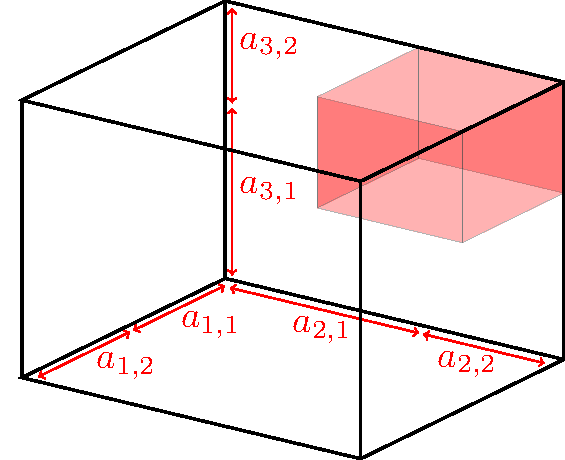
\includegraphics[width=0.4\textwidth]{figures/2/recursion.pdf}
\caption{A recursively constructed $[b_1] \times [b_2] \times [b_3]$ grid, for $n = 2$, $d = 3$.}
\label{fig:recursion}
\end{figure} 

\begin{lem}
\label{lem:recursion}
For $n,d \geq 1$, let $A = (a_{i,j})$ be a $d \times n$ matrix of positive integers, and let $b_i = \sum_{j=1}^n a_{i,j}$, for $1 \geq j \geq d$. Let $S$ be a lethal set under the modified process on $[n]^d$, and for each vertex $\vec{x} = (x_1, \dots, x_v) \in S$, let $T_{\vec{x}}$ be a lethal set on $\prod_{i=1}^d [a_{i,x_i}]$ under $d$-neighbor percolation. Then
$$m(b_1, \dots, b_d, d) \leq \sum_{\vec{x} \in S} |T_{\vec{x}}|.$$
\end{lem}

\begin{proof}
We imagine sub-dividing the $\prod_{i=1}^d [b_{i}]$ brick into smaller blocks by partitioning each of the $d$ axes into segments $a_{i,1}, a_{i,2}, \dots, a_{i,n}$, $1 \leq i \leq d$. Each block is given by a unique product of these segments, and represented by a vector $\vec{x} = (x_1, \dots, x_d) \in [n]^d$. Formally, for each such $\vec{x}$, let $G_{\vec{x}}$ be the block with vertex set
$$\prod_{i=1}^d \{1+ \sum_{j=1}^{x_i -1}a_{i,j}, \dots, \sum_{j=1}^{x_i}a_{i,j} \},$$
and edges between vertices that differ by one in exactly one coordinate. Figure \ref{fig:recursion} illustrates the block $G_{\vec{x}}$ for $\vec{x} = (1,2,2) \in [2]^3$. Observe that $G_{\vec{x}}$ is isomorphic to $\prod_{i=1}^d [a_{i,x_i}]$.

For each $\vec{x} \in S$, let $A_{\vec{x}}$ be the vertices of $G_{\vec{x}}$ corresponding to the vertices of $T_{\vec{x}}$ under isomorphism from $\prod_{i=1}^d [a_{i,x_i}]$ to $G_{\vec{x}}$, and let $A_0 = \cup A_{\vec{x}}$. Observe that $|A_0| = \sum_{\vec{x} \in S} |T_{\vec{x}}|$. We show that $A_0$ is lethal on $\prod_{i=1}^d [b_{i}]$.

By the definition of $T_{\vec{x}}$, for each $\vec{x} \in S$, $A_{\vec{x}}$ is lethal on $G_{\vec{x}}$. Imagine running the $d$-neighbor process until all blocks $G_{\vec{x}}$ are fully infected. We claim that this is sufficient to infect all remaining vertices of $\prod_{i=1}^d [b_{i}]$. Consider the remaining blocks $G_{\vec{x}}$, for $\vec{x} \in [n]^d \setminus S$. Since $S$ is lethal under the modified process, each $G_{\vec{x}}$ is adjacent to fully infected blocks in all $d$ directions. In particular, if we consider expanding out the faces of $G_{\vec{x}}$ towards these infected blocks, the resulting cube has $d$ fully infected faces that share a common corner. By Corollary \ref{cor:three_walls}, this structure will infect all the vertices of $G_{\vec{x}}$. Repeating this process on each uninfected region of $\prod_{i=1}^d [b_{i}]$ (as they are exposed under the modified process) ultimately results in all vertices becoming infected. This completes the proof. 
\end{proof}

% Corollary that shows the recursion produces tight bounds on the size of lethal sets, IF all of the constituent blocks are divisibility cases
We note that although the lemma above is true in full generality, we are only concerned with the particular case where $n=2$ and $d=3$. The following corollary proves that the bound in Lemma \ref{lem:recursion} is tight for $n=2$ and $d=3$, if lethal sets on at least three of the constituent blocks are perfect. 

\begin{cor}
\label{cor:recursion}
Let $A=(a_{i,j})$ be a $3 \times 2$ matrix of positive integers, and let $b_i = a_{i,1} + a_{i,2}$ for all $1 \leq i \leq 3$. Then $m(b_1, b_2, b_3, 3)$ is at most
$$m(a_{1,1}, a_{2,1}, a_{3,1}, 3) +  m(a_{1,2}, a_{2,2}, a_{3,1}, 3) + m(a_{1,2}, a_{2,1}, a_{3,2}, 3) + m(a_{1,1}, a_{2,2}, a_{3,2}, 3).$$
Furthermore, this bound is tight if at least 3 of the constituent grids are perfect. 
\end{cor}

\begin{proof}
The upper bound on $m(b_1, b_2, b_3, 3)$ is a direct consequence of Lemma \ref{lem:recursion}, since $(1,1,1), (2,2,1), (2,1,2), (1,2,2)$ is lethal under the modified process on $[2]^3$. 

If all grids are perfect, then:  
\begin{align*}
&m(a_{1,1}, a_{2,1}, a_{3,1}, 3) +  m(a_{1,2}, a_{2,2}, a_{3,1}, 3) + m(a_{1,2}, a_{2,1}, a_{3,2}, 3) + m(a_{1,1}, a_{2,2}, a_{3,2}, 3) \\[10pt]
&= \frac{a_{1,1}a_{2,1} + a_{2,1}a_{3,1} + a_{3,1}a_{1,1}}{3} + \frac{a_{1,2}a_{2,2} + a_{2,2}a_{3,1} + a_{3,1}a_{1,2}}{3} \\
&\qquad\qquad\qquad\qquad\qquad\qquad\quad + \frac{a_{1,2}a_{2,1} + a_{2,1}a_{3,2} + a_{3,2}a_{2,1}}{3} + \frac{a_{1,1}a_{2,2} + a_{2,2}a_{3,2} + a_{3,2}a_{1,1}}{3} \\[10pt]
&= \frac{(a_{1,1} + a_{1,2})(a_{2,1} + a_{2,2}) + (a_{2,1} + a_{2,2})(a_{3,1} + a_{3,2}) + (a_{3,1} + a_{3,2})(a_{1,1} + a_{1,2})}{3} \\[10pt]
&= \frac{b_1b_2+b_2b_3+b_3b_1}{3}.
\end{align*}
Similarly, suppose, without loss of generality, that $(a_{1,1}, a_{2,1}, a_{3,1})$ is optimal and the remaining grids are perfect. Then:
\begin{align*}
&m(a_{1,1}, a_{2,1}, a_{3,1}, 3) +  m(a_{1,2}, a_{2,2}, a_{3,1}, 3) + m(a_{1,2}, a_{2,1}, a_{3,2}, 3) + m(a_{1,1}, a_{2,2}, a_{3,2}, 3) \\[10pt]
&= \ceil*{\frac{a_{1,1}a_{2,1} + a_{2,1}a_{3,1} + a_{3,1}a_{1,1}}{3}} + \frac{a_{1,2}a_{2,2} + a_{2,2}a_{3,1} + a_{3,1}a_{1,2}}{3} \\
&\qquad\qquad\qquad\qquad\qquad\qquad\quad + \frac{a_{1,2}a_{2,1} + a_{2,1}a_{3,2} + a_{3,2}a_{2,1}}{3} + \frac{a_{1,1}a_{2,2} + a_{2,2}a_{3,2} + a_{3,2}a_{1,1}}{3} \\[10pt]
&= \ceil*{\frac{(a_{1,1} + a_{1,2})(a_{2,1} + a_{2,2}) + (a_{2,1} + a_{2,2})(a_{3,1} + a_{3,2}) + (a_{3,1} + a_{3,2})(a_{1,1} + a_{1,2})}{3}} \\[10pt]
&= \ceil*{\frac{b_1b_2+b_2b_3+b_3b_1}{3}}.
\end{align*}
In both cases, we obtain the lower bound $m(b_1, b_2, b_3, 3)$. This completes the proof. 
\end{proof}

\section{Applying the recursion}

% Handle the divisibility cases, and note that certain augmentations to the recursion allow us to obtain non-divisible optimal grids, if we are cautious with regard to the pieces we use.
Corollary \ref{cor:recursion} provides a proscriptive method for constructing optimal and perfect lethal sets recursively, provided the existence of sufficiently many small building blocks. In the following chapter, we use this technique to obtain perfect lethal sets on all $(b_1,b_2,b_3)$ grids, for $b_1,b_2,b_3 \geq 5$, and optimal lethal sets on all $(b_1,b_2,b_3)$ grids, for $b_1,b_2,b_3 \geq 11$. To facilitate this process, we first present some useful constructions of lethal sets (discussed in greater detail in Chapter [Constructions]), as well as particular applications of Corollary \ref{cor:recursion} that hold for general grids. 

\begin{prop}
\label{prop:3x3xk}
For all $k \geq 1$ such that $k \neq 2$, $(3,3,k)$ is perfect.
\end{prop}

\begin{prop}
For all $k \geq 2$, $(3,6,k)$ is perfect.
\end{prop}

\begin{prop}
For all $k \equiv 3 \pmod 6$ and $l \equiv 1 \pmod 2$, $(3,k,l)$ is perfect.
\end{prop}

Combining the above propositions with Corollary \ref{cor:recursion}, we are able to obtain the following lemmas.

\begin{lem}
Suppose $(b_1, b_2, b_3)$ is optimal. Then $(b_1+3, b_2+3, b_3+3)$ is optimal. 
\end{lem}

\begin{proof}
By Proposition \ref{prop:3x3xk}, each of $(b_1,3,3), (3,b_2,3),(3,3,b_3)$ is perfect. Therefore, by Corollary \ref{cor:recursion}, 
$$m(b_1+3, b_2+3, b_3+3, 3) = m(b_1,b_2,b_3,3) + m(b_1,3,3,3) + m(3,b_2,3,3) + m(3,3,b_3,3),$$
and so $(b_1+3, b_2+3, b_3+3)$ is optimal.
\end{proof}

% Example of the recursion on a small grid and discussion re: the strategies for analyzing percolating sets

\section{Examples and Notation}

% Discuss that the recursion works by assembling any set of compatible n^2 blocks, although it is very rare that it is necessary to use more than 4. 
% Talk about the component pieces necessary to assemble a brick of size (a,b,c).

% Should we talk about the broad behavior of percolating sets?
\section{Regional vs. Temporal Infections}



\chapter{A Tight Bound on Grids of Size $\geq$ 7}

\section{Introduction and Definitions}
Let the ordered tuple $(a,b,c)$ represent the $a \times b \times c$ grid $G$ where $a \geq b \geq c$. We refer to $c$ as the ``thickness" of $G$. For example, the tuple $(5,3,3)$ represents a $5 \times 3 \times 3$ grid of thickness 3. We refer to a tuple as ``divisible", or a ``divisibility case", if and only if $ab+bc+ca \equiv 0 \pmod 3$. Observe that the divisibility cases are precisely those grids with integral lower bounds. The divisibility cases of thicknesses belonging to the three residue classes modulo 3 are illustrated in \{Figure something\}.

In the following lemmas, we use the notation $(a,b,c)+(x,y,z) = (a+x, b+y, c+z)$ to represent respective increases of $x$, $y$, and $z$ to the side lengths $a$, $b$, and $c$ of $G$. We note the following: 
\begin{rem}
By applying the recursion, $(a,b,c)+(x,y,z)$ percolates at the lower bound when either:
\begin{enumerate}
\item $(a,b,c), (a,y,z), (x,b,z), (x,y,c)$ all percolate at the lower bound, or;
\item $(x,y,z), (x,b,c), (a,y,c), (a,b,z)$ all percolate at the lower bound.
\end{enumerate}
\end{rem}

We shall call a thickness ``complete" if it can be shown that all divisibility cases in that thickness percolate at the lower bound. In this section, we demonstrate that thickness 5, thickness 6 and thickness 7 are all complete. As these belong to the residue classes 2, 0, and 1 modulo 3, respectively, we then use a recursive construction to show that all larger grids are also complete. 

\section{Completeness of Thickness 5}
Leveraging \{lemmas from earlier chapters yet to be written\}, we show that all divisibility cases in thickness 5 percolate at the lower bound. 

\begin{lem}
Thickness 5 is complete.
\end{lem}

\begin{proof}
Let $(a,b,2)$ represent an arbitrary (divisible) grid of thickness 2, and let $x = a \pmod 6$ and $y = b \pmod 6$. By \{some as of yet unwritten construction\}, we have that $(a,b,2)$ percolates at the lower bound for all $x,y \in \{0,2,3,5\}$, where $x \neq y$. We consider two constructions: $(a,b,2) + (6,3,3)$ and $(a,b,2) + (6,6,3)$. 

By item (1) of the remark, in order to show that $(a,b,2) + (6,3,3)$ percolates at the lower bound, it is sufficient to show that $(a,b,2), (a,3,3), (6,b,3), (6,3,2)$ all percolate at the bound. By \{more unwritten constructions\}, this is true for all $x,y \in \{0,2,3,5\}$, where $x \neq y$ and at least one of $\{a,b\} > 2$. (Note that if $a=2$, one of the tuples is $(2,3,3)$, which does not percolate at the lower bound; we accommodate for this by re-writing $(a,b,2) + (6,3,3)$ as $(a,b,2) + (3,6,3)$.) The resulting tuple $(a', b', 5)$ is a grid of thickness 5, with $a'$ and $b'$ in the same residue class modulo $6$, and at least one of $\{a',b'\} \geq 9$. From \{some figure representing the divisibility cases of thickness 5\}, we see that the lower bound on $a'$ and $b'$ omits the following three grids: $(5,5,5), (6,6,5)$ and $(8,8,5)$. 

Applying an analogous argument to $(a,b,2) + (6,6,3)$, we must demonstrate that $(a,b,2), (a,6,3), (6,b,3), (6,6,2)$ all percolate at the lower bound. By \{some other constructions\}, we again find that this holds for all $x,y \in \{0,2,3,5\}$, where $x \neq y$ and $a,b > 1$. This gives all thickness 5 tuples $(a',b', 5)$ with $a'$ and $b'$ in different residue classes modulo $6$, where $a',b' \geq 8$. 

SOMETHING IS DIFFERENT

\begin{figure}[]
\centering

\includegraphics[height=1in]{figures/3/test.png}
\end{figure}

\end{proof}

\subsection{Intuition and Statement}

\subsection{Proof}

\chapter{Constructions}

\section{Introduction}

In this chapter, we present diagrammed proofs of lethal sets that percolate at the lower bound. The proofs are organized by the thickness of the grid. Many of the constructions in the following sections belong to infinite families of either optimal or perfect sets. In this case, we shall examine the grids by region, and observe that certain regions can be expanded to arbitrarily large sizes using mathematical induction. 

We shall call a thickness \emph{semi-complete} if all divisibility cases are optimal.

\section{Useful lemmas and observations}

We shall see that similar patterns and structures appear with some regularity in optimal sets. These structures always infect entire regions, and it will be helpful to recognize them within larger grids when they appear. 

\begin{lem}
\label{lem:forest}
Let $G = P_a \Osq P_b$ be a graph and $S \subseteq V(G)$ be a subset of the vertices of $G$. Let $G[\overline{S}]$ be the subgraph of $G$ induced by vertices not in $S$. Then $S$ is a lethal set if and only if $G[\overline{S}]$ is cycle-free, and has no paths between any two boundary vertices. 
\end{lem}

\begin{lem}
\label{lem:three_walls}
Let $G$ be a rectangular prism $(a,b,c)$. If a set $S$ is lethal on three mutually orthogonal faces of $G$, then $S$ is lethal on $G$.
\end{lem}

\begin{cor}
\label{cor:three_walls}
Let $G$ be a grid assembled from sub-grids $G_1, \dots, G_k$. Let $H_1, \dots, H_k$ be sets satisfying the conditions of lemma \ref{lem:three_walls} for sub-grids $G_1, \dots, G_k$, respectively. Then $H = H_1 \cup \dots \cup H_k$ is a lethal set in $G$.
\end{cor}

%\begin{lem}
%\label{lem:unfold}
%Let $G$ be the grid $(a,b,c)$. Let $H$ be a subgraph induced by the vertices of $G$. If the projection of $H$ in the $x$ direction gives the graph $(b,c)$, in the $y$ direction gives $(a,c)$, and in the $z$ direction gives $(a,b)$, and $H$ percolates, then $G$ percolates.
%\end{lem}

%\begin{proof}
%The projection condition guarantees that $G$ has lethal sets on three perpendicular planes. The result follows from lemma \ref{lem:three_walls}.
%\end{proof}

We refer to the union of mutually orthogonal faces of sub-grids $G_1, \dots, G_k$ as a \emph{manifold} of $G$. Therefore, corollary \ref{cor:three_walls} says that if a set $H$ is lethal on the manifold of $G$, then $H$ is lethal in $G$. Furthermore, we define a \emph{proper unfolding} of $G$ as a planar representation of the manifold of $G$. This can be thought of as a special type of folding net of $G$, such that when assembled the resulting structure satisfies the conditions of corollary \ref{cor:three_walls}. 

%\begin{cor}
%\label{cor:unfold}
%Something about unfolding $H$ and its planar embedding. Imagine $H$ as a set of folded up pieces of paper. Let $\mathcal{N}$ be the family of unfolded nets comprising $H$. To show that $G$ percolates, it is sufficient to show that all nets $N \in \mathcal{N}$ harbor lethal infections.
%\end{cor}

\section{Thickness 1}

There are two general constructions in thickness 1 that percolate at the surface area bound. The first construction is perfect for all $(2^n-1, 2^n-1, 1)$ grids, and originates in a 2021 paper by Benevides et al. \cite{benevides:2021}. The second construction is optimal for all grids $(a,b,1)$, where $a \equiv 5 \pmod 6$, $b \equiv 1 \pmod 2$, and $a,b \geq 5$. As such grids constitute non-divisibility cases, this construction is not perfect.

% Purina constructions that percolate at the S.A. bound
\subsection{Purina}

We refer to this construction colloquially as the Purina construction, due to the similarly between its instance on the $(3,3,1)$ grid and the logo of the pet food brand. No funding has been offered, but we are open to the possibility. A more extensive discussion on this pattern can be found in \cite{benevides:2021}.

\begin{con}
\label{con:purina}
All grids of the form $(2^n-1, 2^n-1, 1)$ are perfect.
\end{con}

\begin{figure}[]
\centering

\includegraphics[width=0.1\textwidth]{figures/4/3x3x1.pdf}
\caption{A perfect percolating set for $(3,3,1)$.}
\label{fig:3x3x1}
\end{figure} 

\begin{proof}
This is a recursive construction built from the base component piece shown in figure \ref{fig:3x3x1}. Note that this $(3,3,1)$ construction is lethal under the 3-neighbor bootstrap process, and that it meets the surface area bound:
$$\frac{1}{3} \cdot (ab+bc+ca) = \frac{1}{3} \cdot (9 + 3 + 3) = 5.$$
For larger grids of size $(2^n-1, 2^n-1, 1)$, join four copies of $(2^{n-1}-1, 2^{n-1}, 1)$ about two perpendicular corridors, and infect the vertex at their intersection (figure \ref{fig:15x15x1}). Observe that the resulting set is lethal: each of the four smaller grids is lethal by hypothesis, and the remaining vertices induce a forest with disconnected boundary points, which percolates by lemma \ref{lem:forest}. Furthermore, note that
\begin{align*}
\text{S.A.}(2^n-1,2^n-1,1) &= \frac{1}{3} \cdot (2^{2n}-1) \\
&= 4 \cdot \frac{1}{3} \cdot (2^{2n-2} -1) + 1 = 4 \cdot \text{S.A.}(2^{n-1}-1, 2^{n-1}, 1) + 1,
\end{align*}
and therefore this construction is perfect.
\end{proof}

\begin{figure}[]
\centering
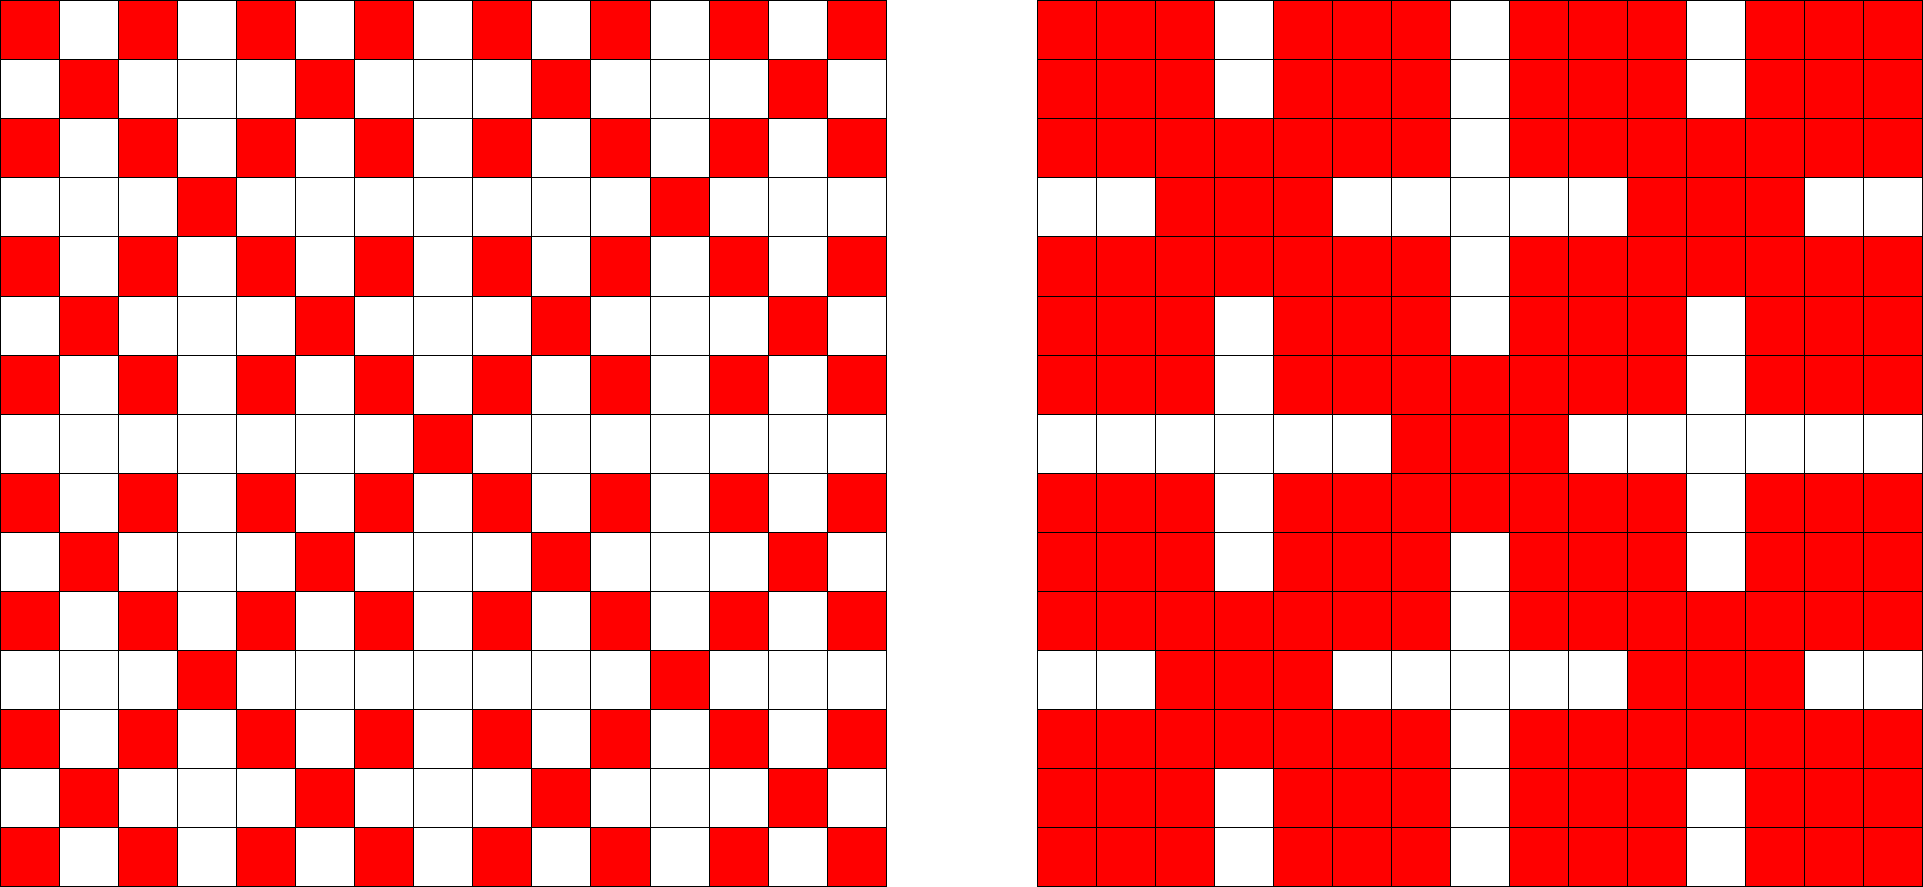
\includegraphics[width=0.6\textwidth]{figures/4/15x15x1.pdf}
\caption{A perfect percolating set for $(15,15,1)$.}
\label{fig:15x15x1}
\end{figure} 

% (odd)x(odd) constructions that percolate at the S.A. bound
\subsection{Snakes}

As indicated by lemma \ref{lem:forest}, a fundamental characteristic of lethal sets $S$ is the presence of an initially uninfected corridor, bounded by walls of infection. This structure is apparent in the second diagrams of figures \ref{fig:15x15x1} and \ref{fig:11x13x1}. These corridors correspond to forests in the complement $G[\overline{S}]$ of $S$. In this subsection, we provide a general method for constructing such corridors in $(a, b, 1)$ grids where $a \equiv 5 \pmod 6$ and $b \equiv 1 \pmod 2$.

% WITH THE EXCEPTION OF WIDTH 3!!!!!
% WIDTH >= 5
\begin{con}
\label{con:snake}
All grids of the form $(a,b,1)$, $a \equiv 5 \pmod 6$, $b \equiv 1 \pmod 2$, and $a,b \geq 5$ are optimal.
\end{con}

\begin{proof}
For grids of the form $(a,b,1)$, $a \equiv 5 \pmod 6$, $b \equiv 1 \pmod 2$, we construct an optimal infected set and show that it percolates by lemma \ref{lem:forest}. For the base case, consider the $(5,5,1)$ grid $G$ illustrated in figure \ref{fig:5x5x1}. Observe that this construction is optimal. Now consider the grid $G'$ resulting from the insertion of a $(5, 2k, 1)$ block, as shown in figure \ref{fig:5x13x1}. Note that the subgraph induced by the uninfected vertices of $G'$ satisfies the conditions of lemma \ref{lem:forest}. Furthermore, note that if any $(5, n, 1)$ grid is optimal, the $(5,n+2,1)$ grid resulting from such a construction has surface area bound $\text{S.A.}(5,n,1) + 4$, which agrees with the number of infected vertices.

\begin{figure}[]
\centering
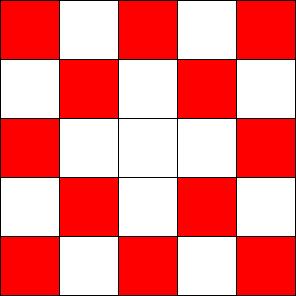
\includegraphics[width=0.15\textwidth]{figures/4/5x5x1.pdf}
\caption{An optimal percolating set for $(5,5,1)$.}
\label{fig:5x5x1}
\end{figure} 

\begin{figure}[]
\centering
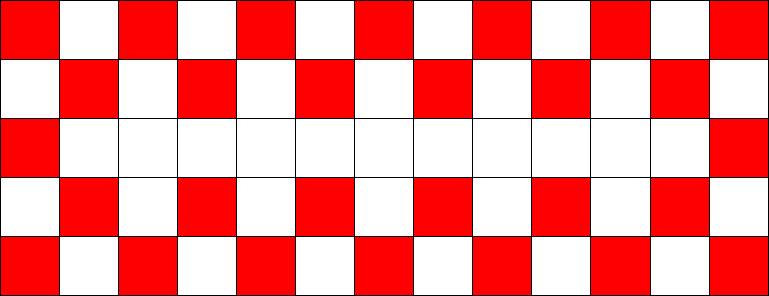
\includegraphics[width=0.5\textwidth]{figures/4/5x13x1.pdf}
\caption{An optimal percolating set for $(5,13,1)$.}
\label{fig:5x13x1}
\end{figure} 

To extend this construction in the vertical direction, we introduce a kink in the snaking infection. This kink requires six rows to produce a repeating pattern. The structure of this design is shown in figure \ref{fig:11x13x1}. For grids of smaller width, the same construction gives optimal percolating sets; however, the snaking pattern is increasingly difficult to recognize in thin grids.
\end{proof}

\begin{figure}[]
\centering

\includegraphics[width=0.6\textwidth]{figures/4/11x13x1.pdf}
\caption{An optimal percolating set for $(11,13,1)$.}
\label{fig:11x13x1}
\end{figure} 

% Maybe other (divisibility) constructions that percolate at 1 over the bound (if they exist)?

\section{Thickness 2}

In this section we examine four infinite families of perfect grids. We show that each has a manifold that admits a lethal set of perfect size. We note that such lethal sets are likely to exist for nearly all divisibility cases in thickness two; however, constructions are elusive and those presented here are sufficient to prove the main result of this thesis.

% (0 mod 6, 3, 2)
\begin{con}
All $(a,3,2)$ grids with $a \equiv 0 \pmod 6$ are perfect. 
\end{con}

\begin{figure}[]
\centering
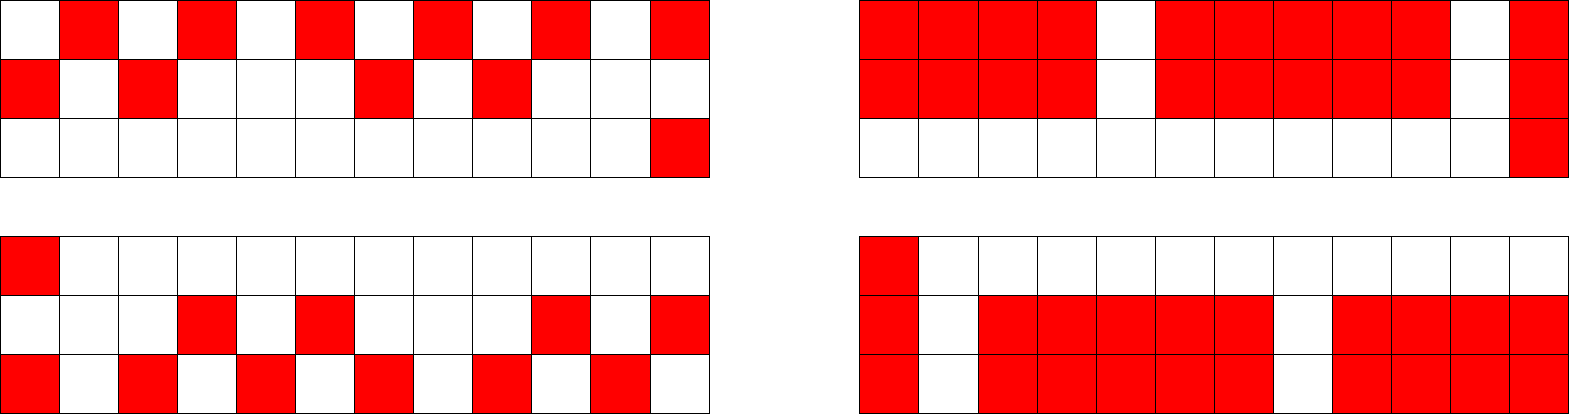
\includegraphics[width=0.8\textwidth]{figures/4/3x12x2.pdf}
\caption{A perfect percolating set for $(3,12,2)$.}
\label{fig:3x12x2}
\end{figure} 

\begin{figure}[]
\centering
%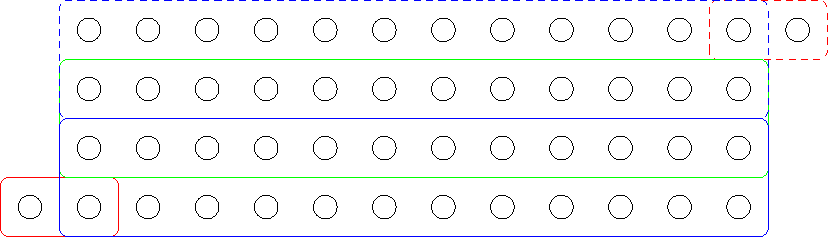
\includegraphics[width=0.6\textwidth]{figures/4/3x12x2_manifold.pdf}
\caption{A proper unfolding of $G= (3,12,2)$. Colored rectangles indicate faces of $G$. Dashed lines indicate that cells appear on different layers. }
\label{fig:3x12x2_manifold}
\end{figure} 

\begin{figure}[]
\centering
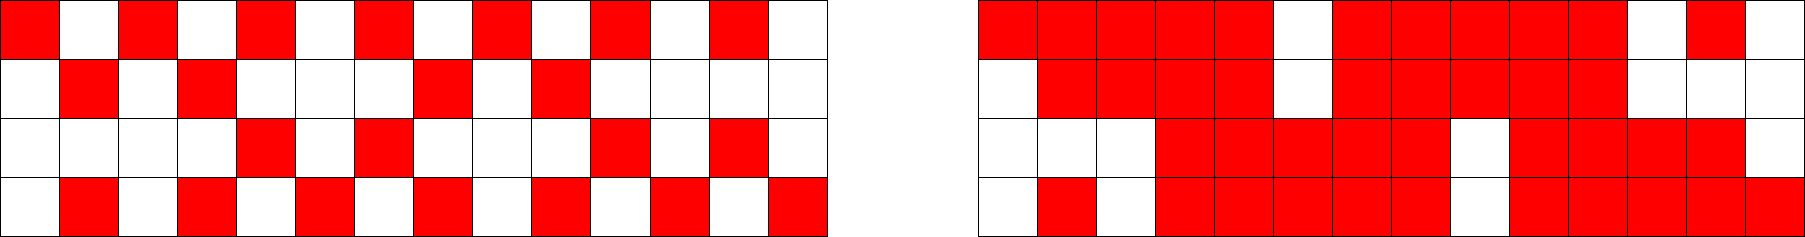
\includegraphics[width=0.8\textwidth]{figures/4/3x12x2_unfolded_lethal.pdf}
\caption{A percolating set on the proper unfolding of $G= (3,12,2)$.}
\label{fig:3x12x2_unfolded_lethal}
\end{figure} 

\begin{proof}
\end{proof}

% (3 mod 6, 3, 2)
\begin{con}
All $(a,3,2)$ grids with $a \equiv 0 \pmod 6$ are perfect. 
\end{con}

\begin{proof}
\end{proof}

% (2 mod 6, 5 mod 6, 2)

% a,b, MUST BE A CERTAIN SIZE
\begin{con}
All $(a,b,2)$ grids with $a,b \in \{2,5\} \pmod 6$ and $a \neq b \pmod 6$ are perfect. 
\end{con}

\begin{figure}[]
\centering
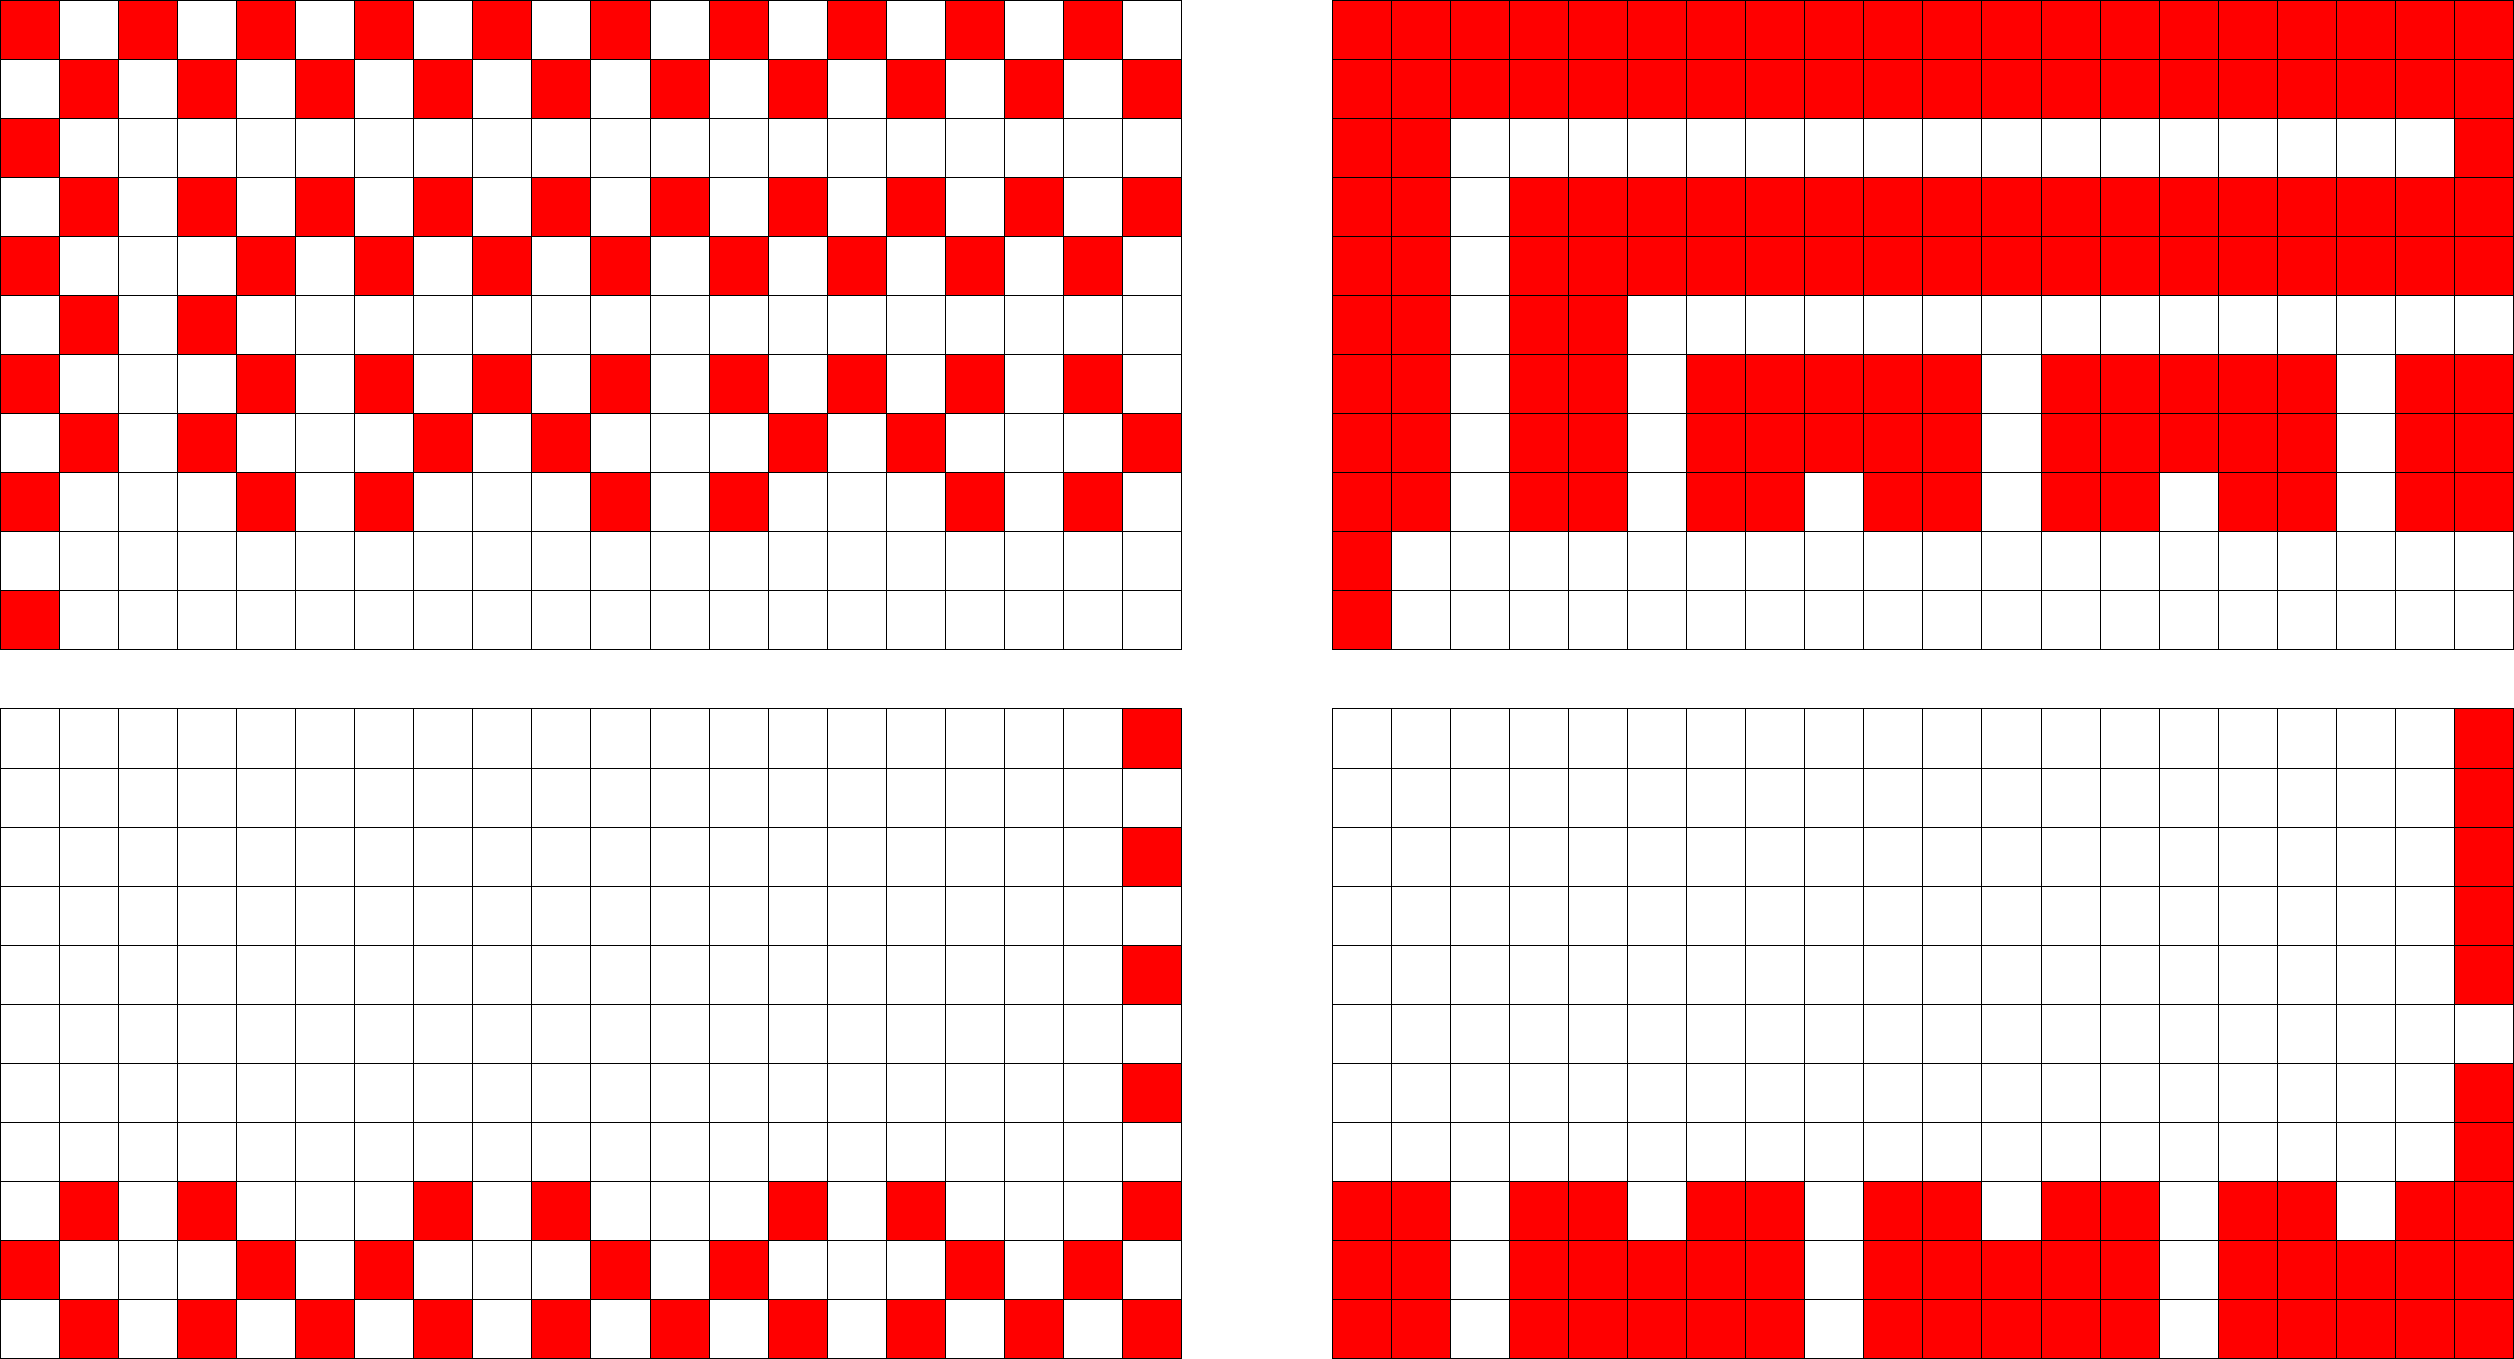
\includegraphics[width=0.8\textwidth]{figures/4/11x20x2.pdf}
\caption{A perfect percolating set for $(11,20,2)$.}
\label{fig:11x20x2}
\end{figure} 

\begin{figure}[]
\centering
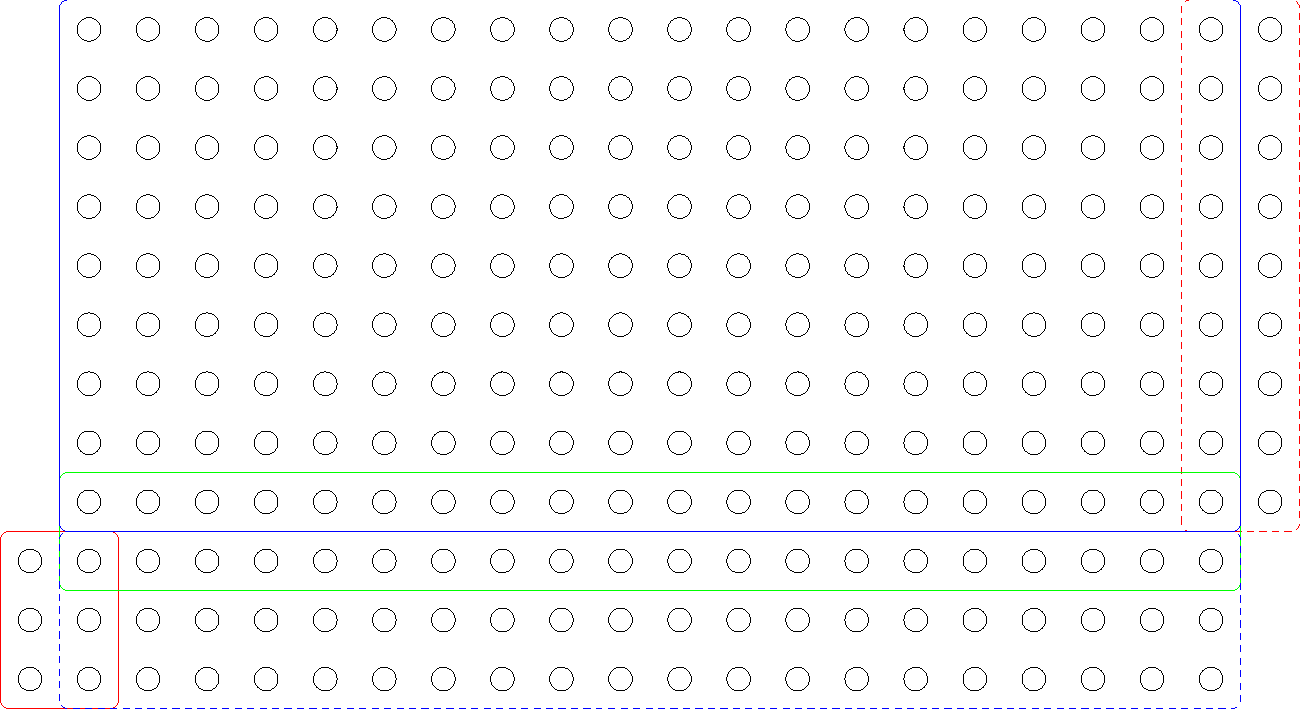
\includegraphics[width=0.6\textwidth]{figures/4/11x20x2_manifold.pdf}
\caption{A proper unfolding of $G= (11,20,2)$. Colored rectangles indicate faces of $G$. Dashed lines indicate that cells appear on different layers. }
\label{fig:11x20x2_manifold}
\end{figure} 

\begin{figure}[]
\centering
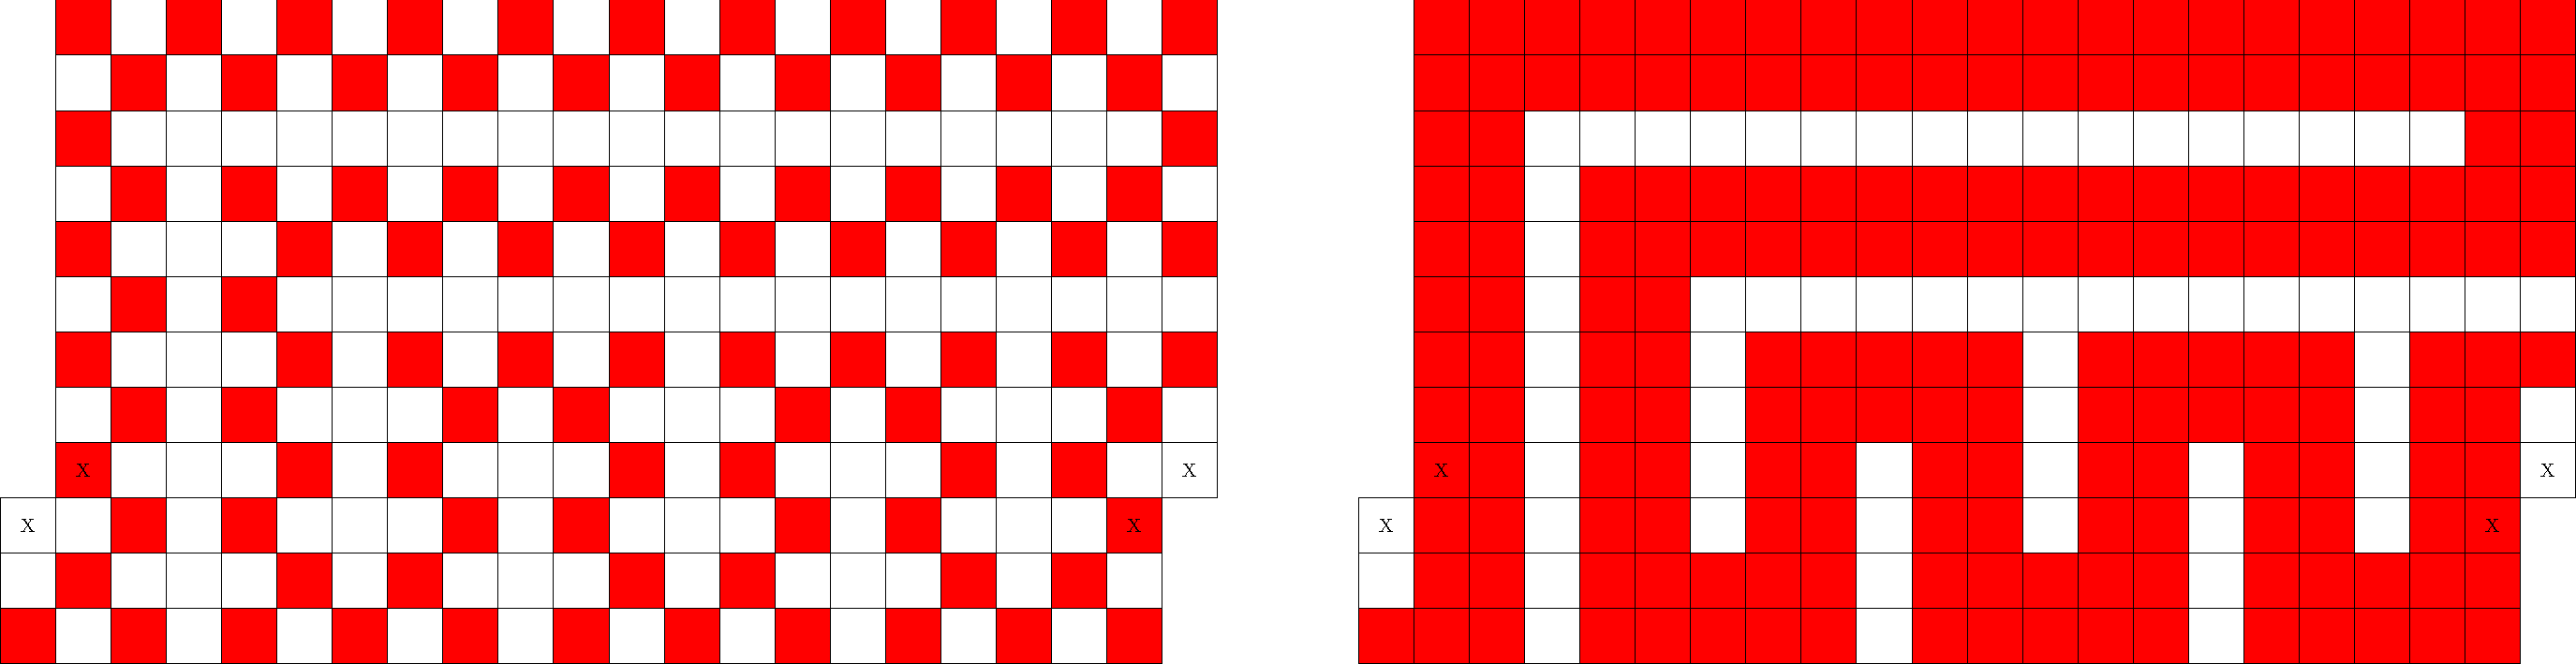
\includegraphics[width=0.8\textwidth]{figures/4/11x20x2_unfolded_lethal.pdf}
\caption{A percolating set on the proper unfolding of $G= (11,20,2)$.}
\label{fig:11x20x2_unfolded_lethal}
\end{figure} 

\begin{proof}
Let $G$ be an $(a,b,2)$ grid with $a,b \in \{2,5\} \pmod 6$ and $a \neq b \pmod 6$, and let $H$ be an unfolding of $G$ (figure \ref{fig:11x20x2_manifold}). We show that this unfolding is proper, and that it admits a perfect lethal set. 

The above construction holds for $a \geq 11$ and $b \geq 8$. SAY SOMETHING ABOUT THE MISSING CASES.
\end{proof}

% (3 mod 6, 0 mod 6, 2) 

% a,b MUST BE A CERTAIN SIZE
\begin{con}
All $(a,b,2)$ grids with $a,b \in \{0,3\} \pmod 6$ and $a \neq b \pmod 6$ are perfect. 
\end{con}

\begin{proof}
Consider the $(21,12,2)$ grid $G$ shown in figure \ref{fig:12x21x2}. Let $H$ be a unfolding of $G$ (figure \ref{fig:12x21x2_unfolded}). Observe that $H$ is proper: three mutually orthogonal faces of $G_1$ are shown by blue, green and dashed red regions, and mutually orthogonal faces of $G_2$ are shown by the red, green and dashed blue regions. We show that $H$ admits a lethal set of size $\text{S.A.}(12,21,2) = 106$. Consider such a set, as shown in figure \ref{fig:12x21x2_unfolded_lethal}. (Observe that this is the same set as shown in figure \ref{fig:12x21x2}.) By lemma \ref{lem:forest}, this set percolates with the exception of two $C_4$s in the top and bottom of the grid. However, notice that one of these cells is a duplicate of an already infected cell. (This duplication is a consequence of the proper unfolding of $G$.) Therefore, $H$ admits a lethal set, and by corollary \ref{cor:three_walls}, $G$ is perfect.

For all larger grids, observe that the snaking corridor in the left side $G$ can be extended by multiples of 6 in both the $x$ and $y$ directions. These resulting grid still percolates under lemma \ref{lem:forest}. A simple calculation verifies that such an alteration produces initial infections at the surface area bound. 
\end{proof}

\begin{figure}[]
\centering
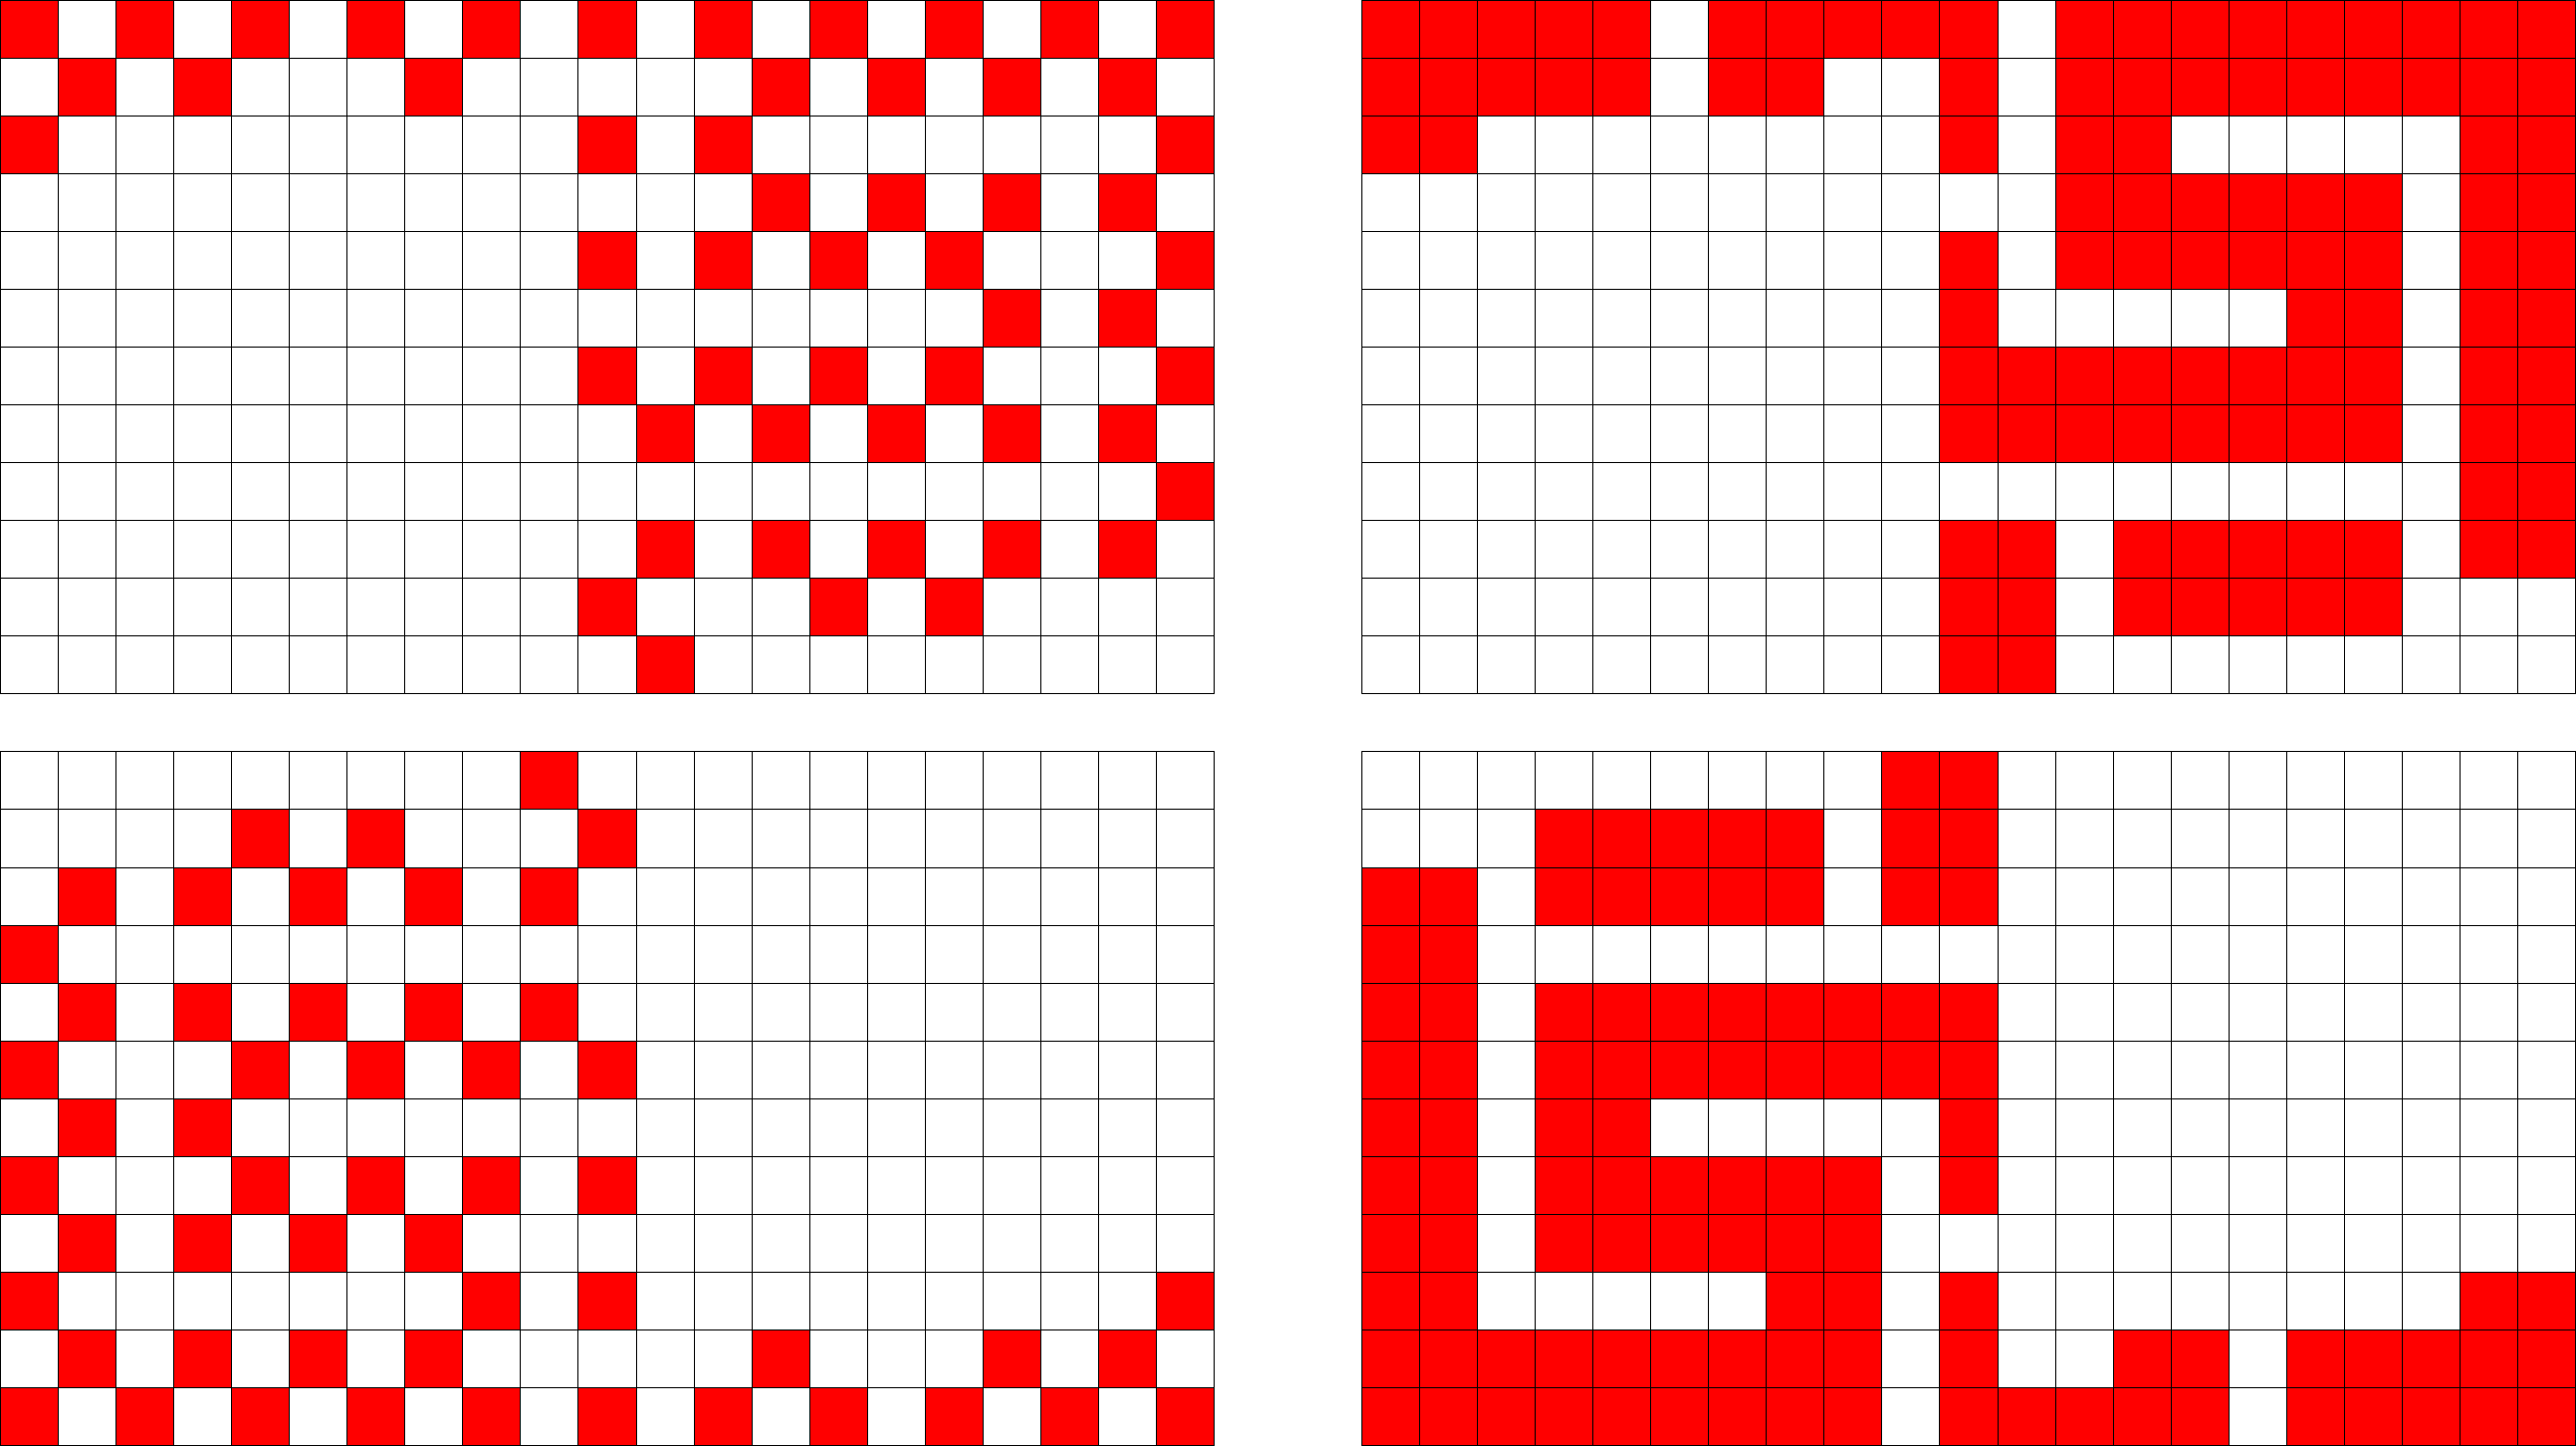
\includegraphics[width=0.8\textwidth]{figures/4/12x21x2.pdf}
\caption{A perfect percolating set for $(12,21,2)$.}
\label{fig:12x21x2}
\end{figure} 

\begin{figure}[]
\centering
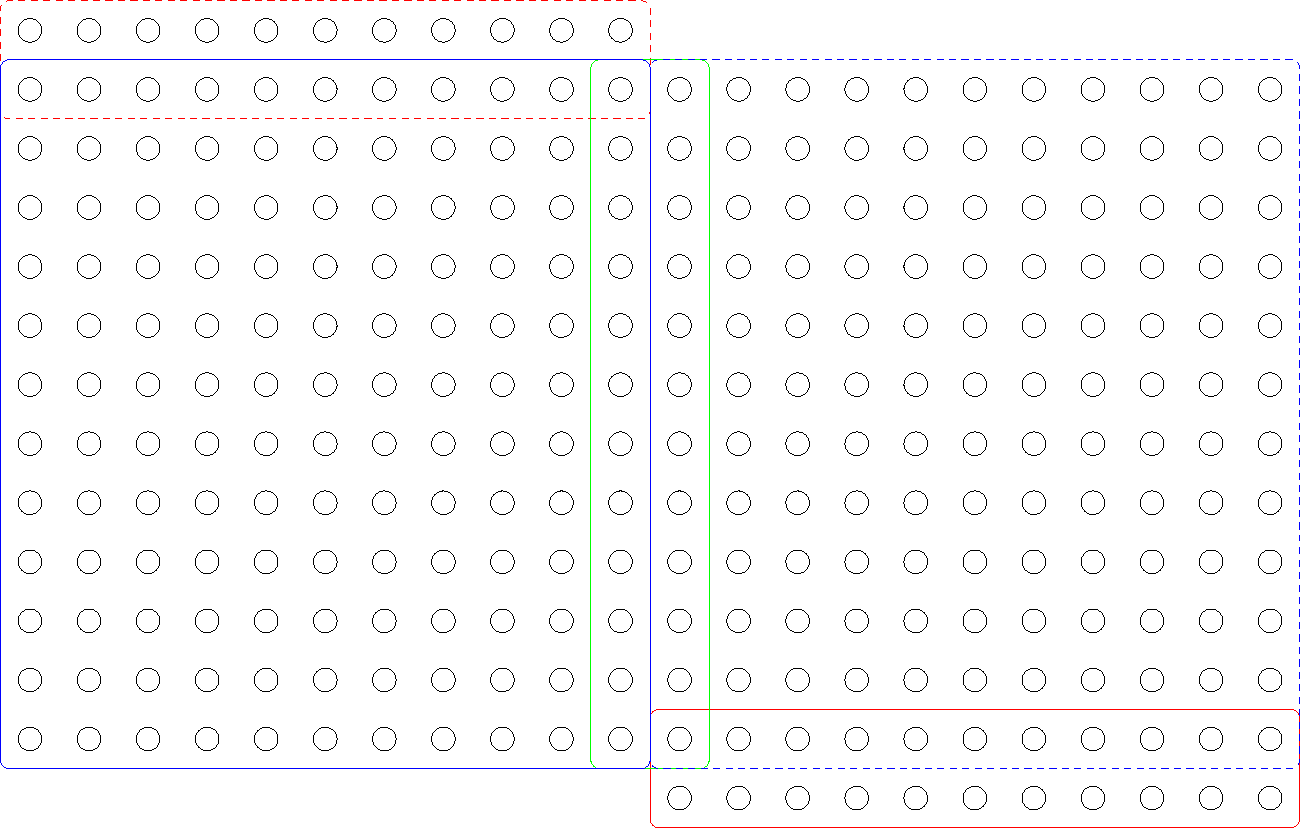
\includegraphics[width=0.6\textwidth]{figures/4/12x21x2_unfolded.pdf}
\caption{A proper unfolding of $G= (12,21,2)$. Colored rectangles indicate faces of $G$. Dashed lines indicate that cells appear on different layers. }
\label{fig:12x21x2_unfolded}
\end{figure} 

\begin{figure}[]
\centering
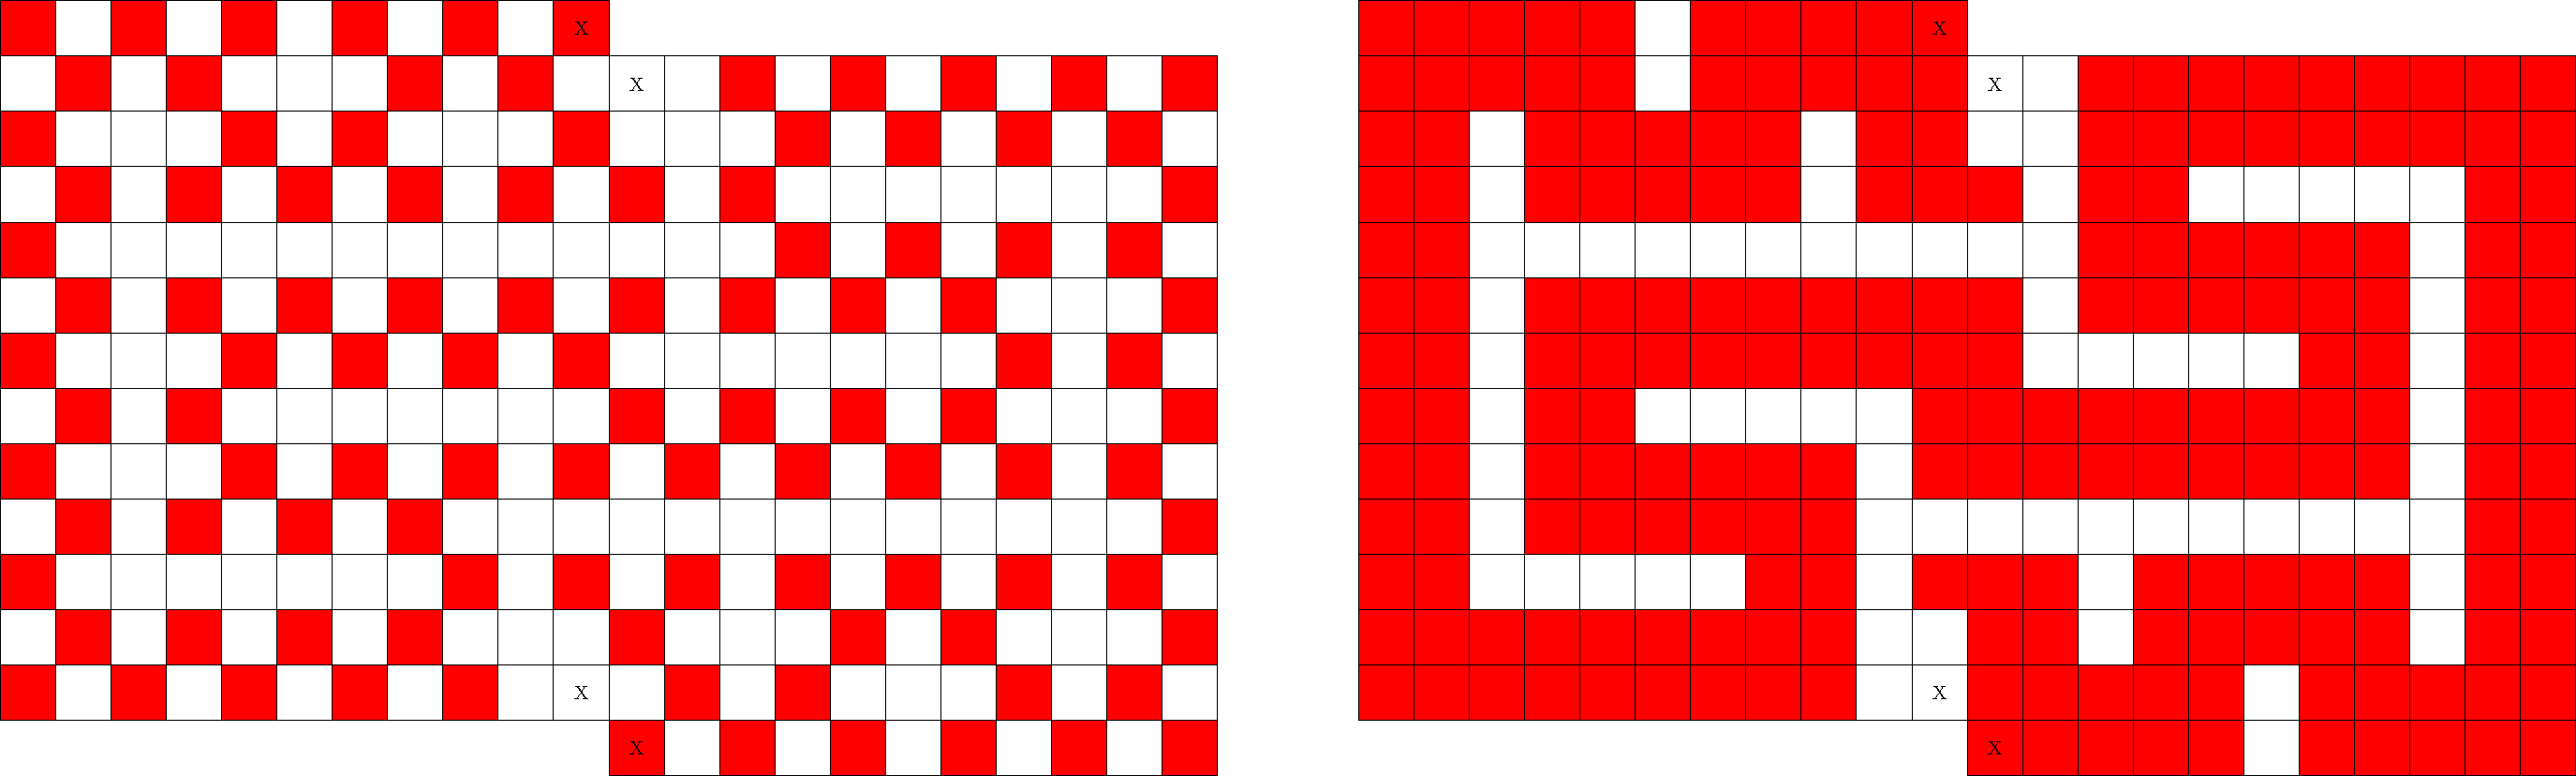
\includegraphics[width=0.8\textwidth]{figures/4/12x21x2_unfolded_lethal.pdf}
\caption{A percolating set on the proper unfolding of $G= (12,21,2)$.}
\label{fig:12x21x2_unfolded_lethal}
\end{figure} 

\section{Thickness 3}

\begin{con}
All $(a,b,3)$ grids $G$ with $a \equiv 3 \pmod 6$ and $b \equiv 1 \pmod 2$ are perfect. 
\end{con}

\begin{proof}
Consider the grid $H=(a+2,b+2,1)$, and observe that such a grid admits an optimal percolating set by construction \ref{con:snake}. Note that
$$\text{SA}(a,b,3) = \ceil{\text{SA}(a+2,b+2,1)} - 3.$$
We show that an unfolding of $G$ can be obtained from a simple augmentation of $H$. Let $H'$ be the grid obtained by deleting the four vertices in the bottom, right-most corner of $H$ (see figure \ref{fig:17x25x1_unfolded}). Consider the folding pattern illustrated in figure \ref{fig:17x25x1_manifold}, and observe that the pairs of vertices adjacent to the deleted region are duplicates of each other. (In other words, consider folding up the red and green regions in figure \ref{fig:17x25x1_manifold}, and notice that this operation causes vertices to overlap.) Taking this into account, the unfolding of $G$ percolates by lemma \ref{lem:forest}. Since $H$ admits an optimal percolating set of size $\ceil{\text{SA}(a+2,b+2,1)}$, and precisely 3 of the vertices deleted from $H$ to obtain $H'$ were infected, it follows that the unfolding of $G$ percolates at the lower bound. Finally, by lemma \ref{lem:three_walls}, since the unfolding of $G$ is proper and percolates at the lower bound, $G$ is perfect.
\end{proof}

\begin{figure}[]
\centering

\includegraphics[width=0.8\textwidth]{figures/4/17x25x1_unfolded.pdf}
\caption{A percolating set on the proper unfolding $H'$ of $G= (15,23,3)$.}
\label{fig:17x25x1_unfolded}
\end{figure}

\begin{figure}[]
\centering
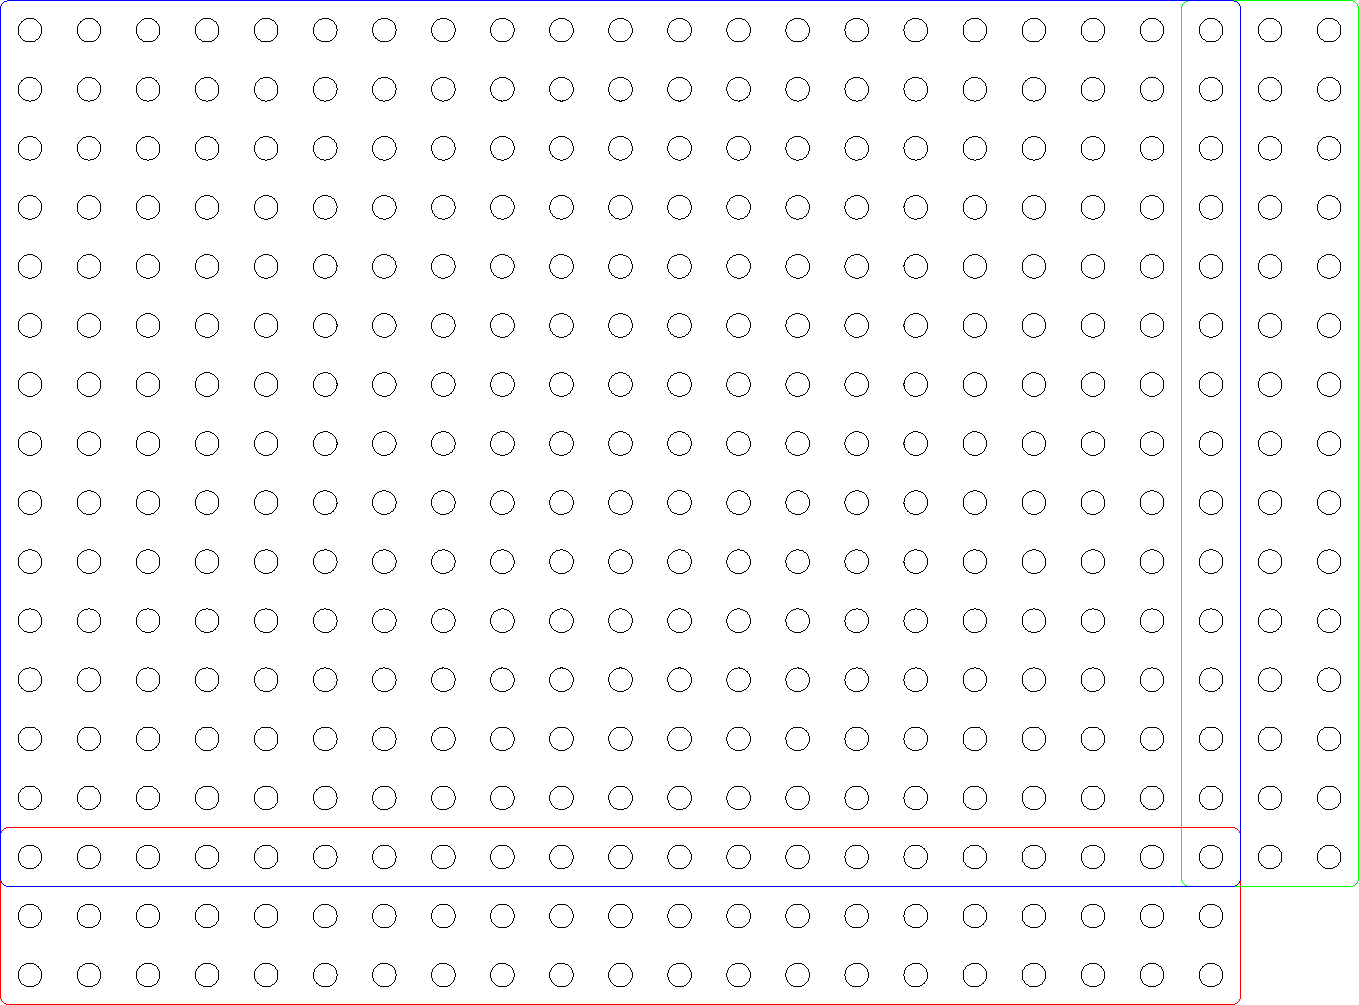
\includegraphics[width=0.6\textwidth]{figures/4/17x25x1_manifold.pdf}
\caption{A proper unfolding of $G= (15,23,3)$. Colored rectangles indicate faces of $G$. }
\label{fig:17x25x1_manifold}
\end{figure}

% (5, 3, 3)

% (5, 2, 2) 

% (5, 5, 5)

% (8, 5, 5)

% (a, 3, 3)

% (6, 3, 3)

% (6, 3, 2)

\begin{figure}[]
\centering
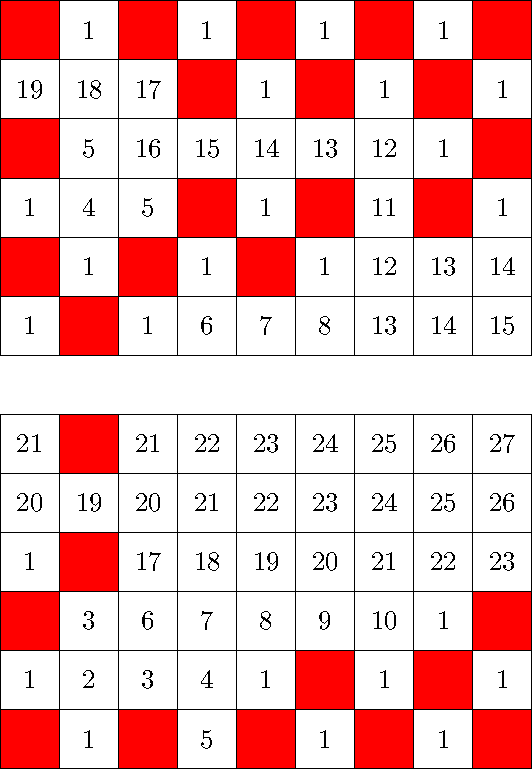
\includegraphics[width=\textwidth]{figures/4/6x9x2_numbered_heatmap.pdf}
\caption{}
\label{fig:6x9x2}
\end{figure} 

\begin{figure}[]
\centering
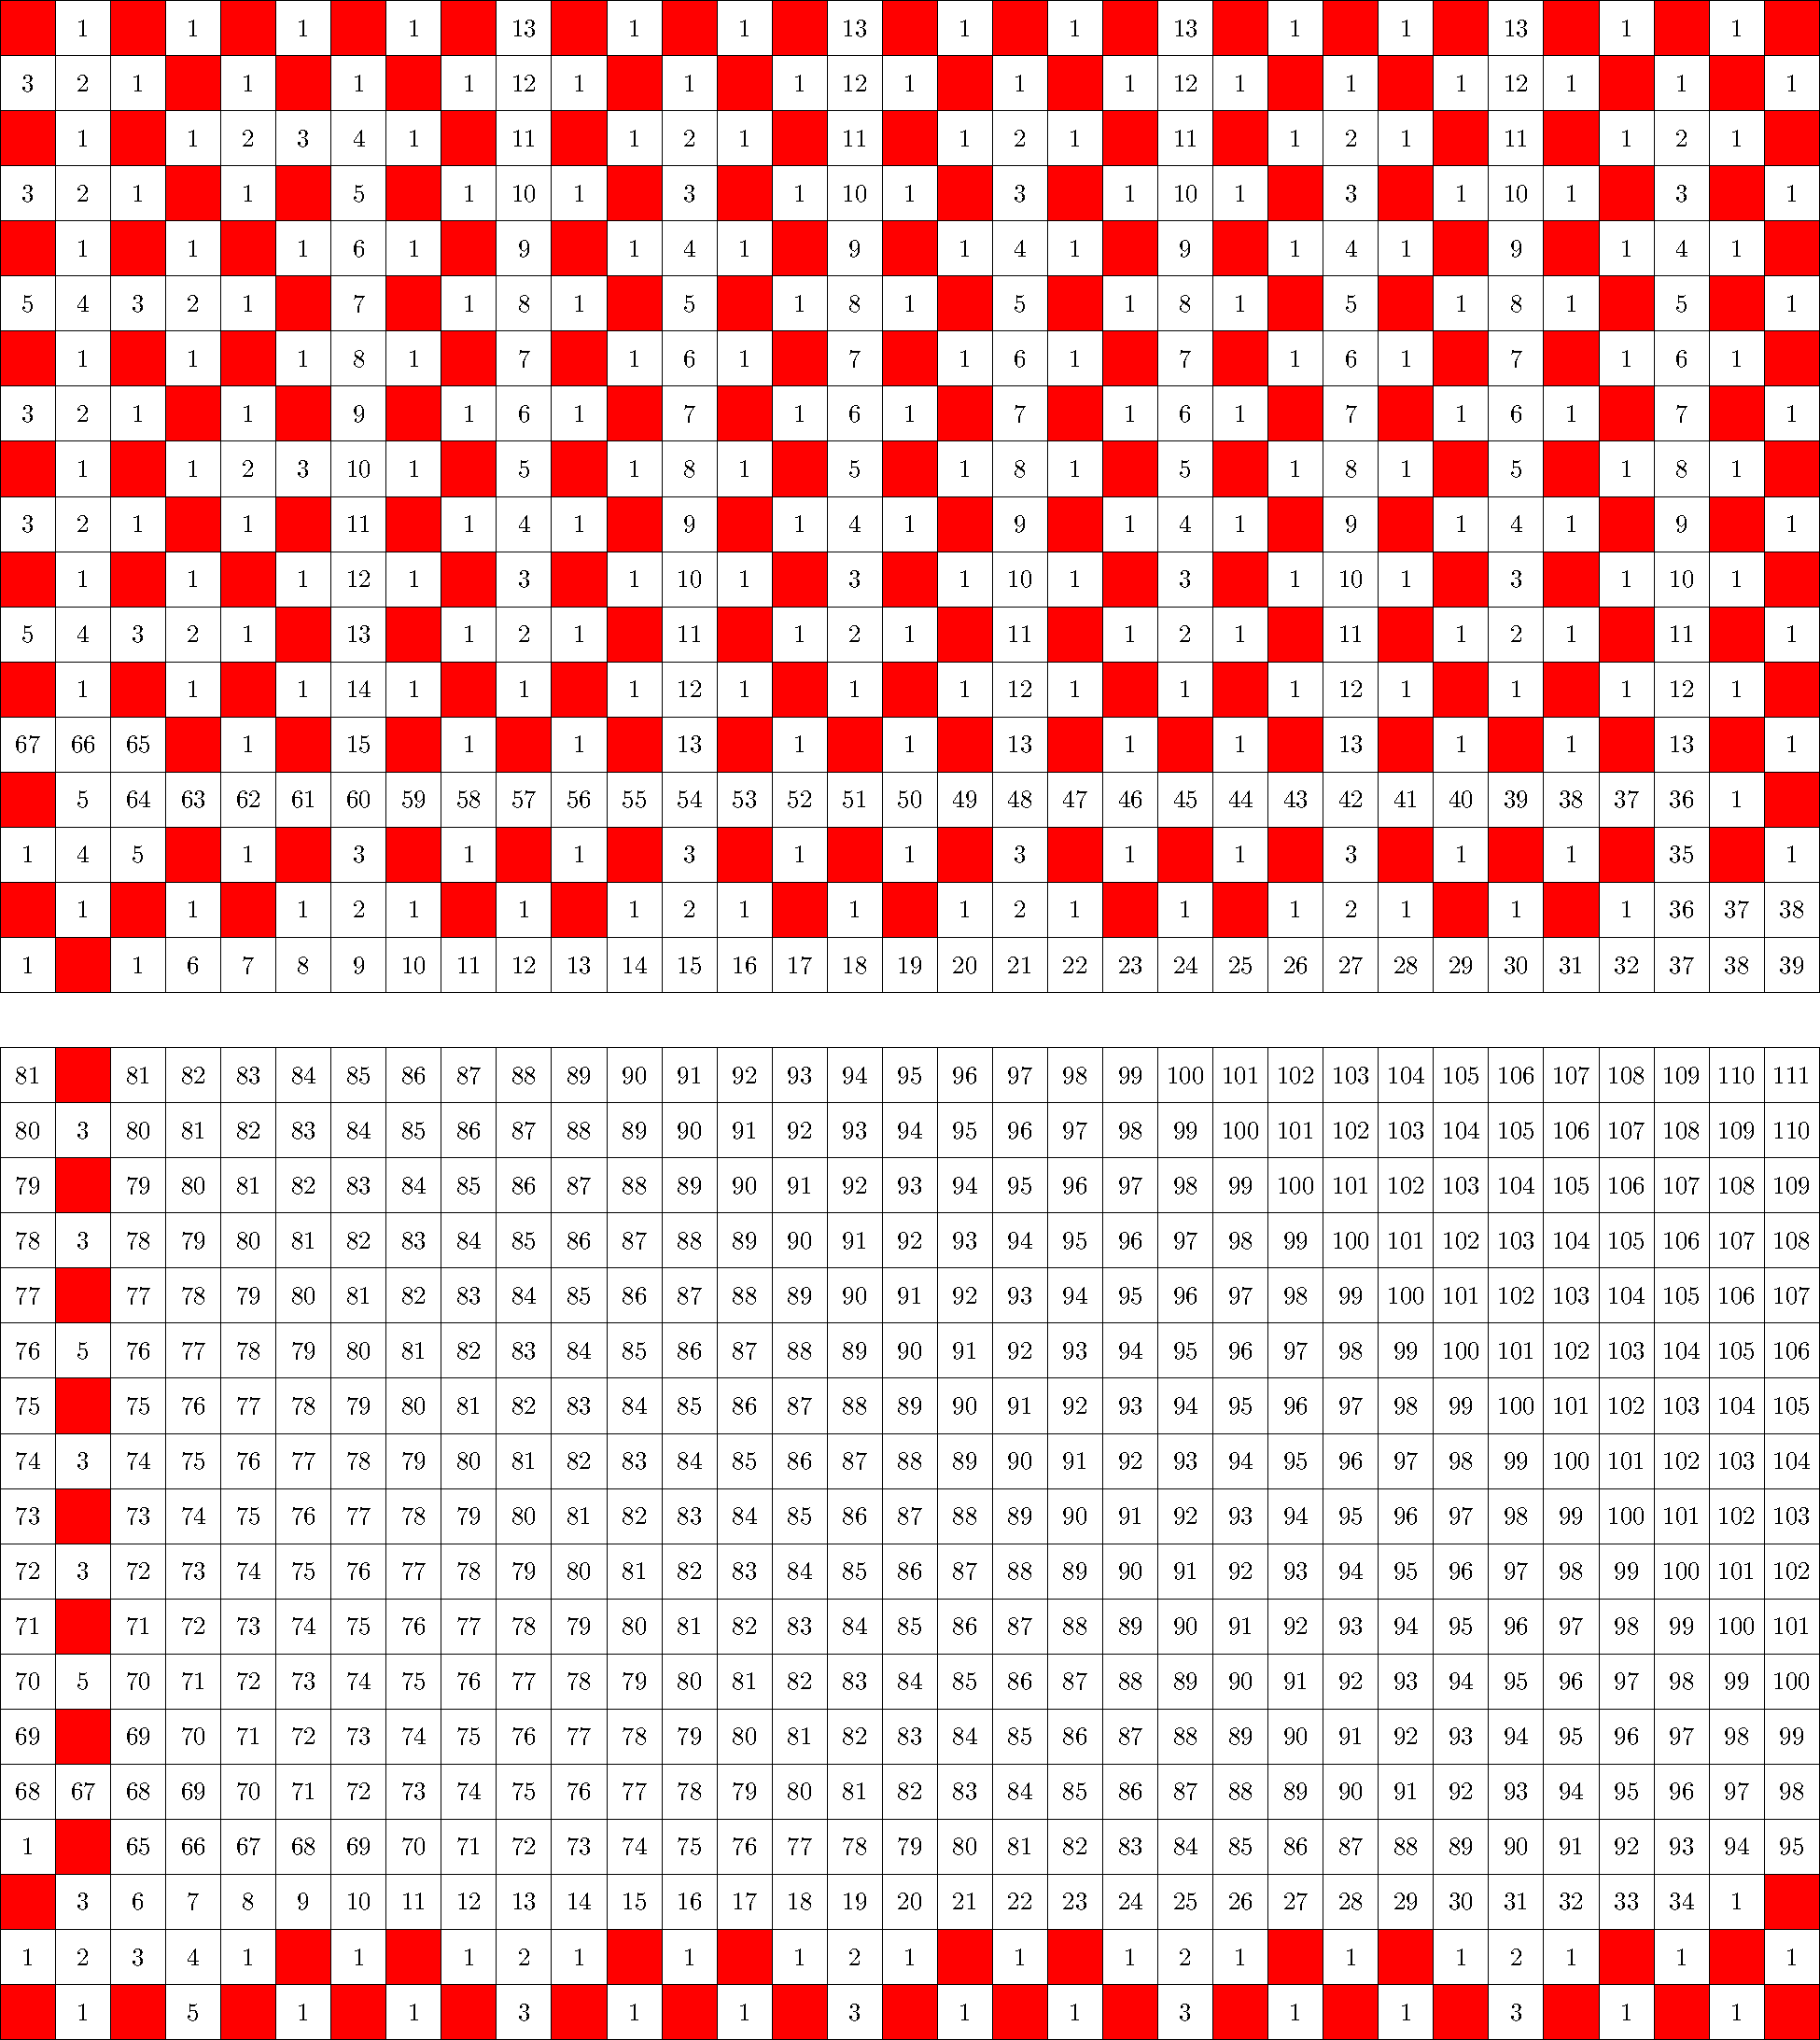
\includegraphics[width=\textwidth]{figures/4/18x33x2_numbered_heatmap.pdf}
\caption{}
\label{fig:6x9x2}
\end{figure} 



\chapter{Torus}

\section{Introduction}

I know I shouldn't be working on this now but I have some ideas. We can use Benevides proof of the lower bound for the torus, which states the following:

\begin{lem}
Let $T = C_n \Osq C_m$ be the $n \times n$ torus. Let $A$ be a lethal set on $T$. Then $|A| \geq \frac{nm + c}{3}$, where $c$ is the number of components in the graph $T[\overline{A}]$. 
\end{lem}

There are some nice observations to be made here. First, in much the same way that loss of surface area contributes to fractional increases in the surface area bound for grid graphs, the number of components can be understood to indicate sub-optimality in the torus. As a particular example, the torus $T = C_18 \Osq C_12$ has lower bound of $72.33$. This can be obtained from an optimal (but not perfect) thickness one grid construction for $(17,11,1)$, with an additional vertex in the bottom rightmost corner. 

There's something interesting happening here. In this particular case, $T[\overline{A}]$ has three components. Assuming the best case scenario (where it has one component), we get the lower bound of 72.33. However, if we instead consider three components, the lower bound sits precisely as 73. As the construction of $T$ simple involves adding an additional vertex to an optimal (not perfect) grid construction, it appears as though the inadequacies of the grid construction (namely, cells that are infected by 4 neighbors) somehow translate directly to inadequacies of the torus construction (multiple components in the complement). 

Oh wait, is this just because the surface area argument is fundamentally an argument about the number of components in the complement? I think it is. Every time you lose surface area, you've deleted a tree from the forest (because in order to remove the final vertex in a tree, you need an inefficiency--unless the tree sits on the boundary). Therefore, it makes sense that the best solutions on the torus have exactly one component in the complement.

How does the surface area argument map to an argument about components? Knowing this should allow us to construct a lower bound on the 4D torus.

There are other questions regarding some form of algebraic or numerical equivalence between expressions for the lower bounds of tori and grids. It is clear that 

% etc.


%--------------------------------------------------------------------------------------%
%								BIBLIOGRAPHY										
%--------------------------------------------------------------------------------------%

\backmatter % Makes the Bibliography an unnumbered section (and implements appropriate page breaks).
	\addtoToC{Bibliography}
	\bibliographystyle{abbrv} % Choose the style that you want to use (or your supervisor wants you to use).
	\bibliography{refs} % Use your bibtex file. 

\end{document}
